% Copyright (c) 2005-2009 Center for Urban Simulation and Policy Analysis,
% University of Washington.  Permission is granted to copy, distribute and/or
% modify this document under the terms of the GNU Free Documentation License,
% Version 1.2 or any later version published by the Free Software Foundation;
% with no Invariant Sections, no Front-Cover Texts, and no Back-Cover Texts.
% A copy of the license is included in the section entitled "GNU Free
% Documentation License".

\chapter{The \package{urbansim} Opus Package}

\section{Introduction}

This chapter describes the different components --- datasets and models ---
contained in the \package{urbansim} package. 

\section{Datasets}
\label{sec:urbansim-datasets}
 
%
All datasets defined in \package{urbansim} are implemented as children of the
Opus \package{opus_core} class \class{Dataset} described in
Section~\ref{sec:opus-core-datasets}. Each dataset sets default values for several
class properties, such as a name of the unique identifier (\verb|id_name|),
dataset name (\verb|dataset_name|), \verb|in_table_name| and
\verb|out_table_name|. For example, the following code 
\begin{verbatim}
>>> from opus_core.datasets.dataset import Dataset
>>> households = Dataset(in_storage = storage,
                         id_name='household_id',
                         dataset_name='household',
                         in_table_name='households', 
                         out_table_name='households')
\end{verbatim}
is equivalent to
\begin{verbatim}
>>> from urbansim.datasets.household_dataset import HouseholdDataset
>>> households = HouseholdDataset(in_storage = storage)
\end{verbatim}

The \package{urbansim} datasets are defined in \verb|urbansim.datasets|. 
We use the following naming convention: For module name we use the dataset 
name in lower case in singular form, where single words are connected by
'_', and ending with ``_dataset''.
For class name we capitalize the first letters in each word of the dataset 
name, use singular form and add 'Dataset' at the end. For example, a dataset for
development projects is defined in class \class{DevelopmentProjectDataset}
implemented in the module \file{development_project_dataset.py}. For interaction
sets, we connect the two dataset names in the same way, but with 
an 'x' in the module name and an 'X' in the class name. For example, an
interaction set of development projects and gridcells is defined in
\class{DevelopmentXProjectGridcellDataset} implemented in
\file{development_project_x_gridcell_dataset.py}.

\subsection{Predefined Datasets}
 
%
Table~\ref{tab:urbansim-datasets} lists dataset classes that are predefined in
\package{urbansim} (in alphabetical order), including the default value for
\verb|dataset_name|, \verb|in_table_name|, \verb|id_name| and name of the
module in which the class is implemented (excluding '.py'). In most cases they
correspond to database tables described in
Chapter~\ref{chapter:urbansim-database-tables}. The corresponding table name
is the value of \verb|in_table_name|.

%begin{latexonly}
%end{latexonly}
\begin{table}
\begin{center}
\begin{tabular}{|l||l||l|}\hline
\multicolumn{1}{|c||}{dataset_name} & \multicolumn{1}{c||}{in_table_name (default)}&
\multicolumn{1}{c|}{id_name (default)} \\\hline\hline
%
building & buildings & building_id 
\\
building_type & building_types & building_type_id 
\\
city* & cities & city_id 
\\  
county* & counties & county_id 
\\
development_constraint & development_constraints & constraint_id 
\\ 
development_event & development_events & grid_id, scheduled_year 
\\
development_event_history & development_event_history & grid_id, scheduled_year 
\\
development_group & development_type_groups & group_id 
\\
development_project & -- & project_id 
\\
development_type & development_types, & development_type_id 
\\
& development_type_group_definitions & 
\\
employment_control_total & annual_employment_control_totals & year, sector_id 
\\
employment_sector  & employment_sectors & sector_id
\\
employment_sector_group & employment_adhoc_sector_groups & group_id 
\\
faz* & fazes & faz_id 
\\
fazdistrict* & -- & fazdistrict_id 
\\
gridcell* & gridcells & grid_id 
\\
household & households & household_id
\\
household_characteristic & household_characteristics_for_ht & --
\\
household_control_total & annual_household_control_totals & year 
\\
job & jobs & job_id 
\\
job_building_type & job_building_types & id 
\\
large_area* & large_areas & large_area_id 
\\
neighborhood* & neighborhoods & neighborhood_id 
\\
plan_type & plan_types & plan_type_id 
\\
plan_type_group & plan_type_groups & group_id 
\\
race & race_names & race_id 
\\
rate (households) & annual_relocation_rates_for_households & age_min, income_min 
\\
rate (jobs) & annual_relocation_rates_for_jobs & sector_id 
\\
region & regions & region_id 
\\
ring & rings & ring_id 
\\
target_vacancy & target_vacancies & year
\\
travel_data & travel_data & from_zone_id, to_zone_id 
\\
urbansim_constant & urbansim_constants & --
\\
vacant_land_and_building_type & building_types & building_type_id 
\\
zone* & zones & zone_id 
\\\hline
\end{tabular}
\end{center}
\caption{\label{tab:urbansim-datasets}Datasets defined in \package{urbansim}. A dataset
  marked with * is a location set, i.e. it represents a set of locations of
  a specific geographical unit and can be visualized as a two-dimensional image.}
\end{table}
%begin{latexonly}
%end{latexonly}

In addition, they are a few interaction sets defined in \package{urbansim},
listed in Table~\ref{tab:urbansim-interaction-datasets}. The dataset name of
such interaction set is created automatically from the names of the two
interacting datasets. Note that for standard usage, there is no need to explicitely define
an interaction set for every two specific datasets. 
If a specific definition is not found, Opus framework creates an abstract interaction set
using the \class{InteractionDataset} in \package{opus_core} (see Section~\ref{sec:interaction-set}).

\begin{table}
\begin{center}
\begin{tabular}{|l|}\hline
\multicolumn{1}{|c|}{dataset_name}  \\\hline\hline
development_project_x_gridcell \\
household_x_gridcell \\
household_x_neighborhood \\
household_x_zone \\
job_x_gridcell \\\hline
\end{tabular}
\end{center}
\caption{\label{tab:urbansim-interaction-datasets}Interaction datasets defined
  in \package{urbansim}. }
\end{table}

\section{Variables}

%
Variables predefined in \package{urbansim} are structured according to the
dataset to which they belong. They are implemented in directories of the same
name as \verb|dataset_name| which is placed in the top directory of
\package{urbansim}. For example, all gridcell variables are placed in
\file{urbansim/gridcell}, all interaction variables of households and
gridcells are placed in \file{urbansim/household_x_gridcell}. All variables
are defined as children of the \package{opus_core} class \class{Variable} or as expressions in \file{alias.py} file,
 and thus, they follow the guidelines presented in Section~\ref{sec:opus-variable}.

\section{Models}
\label{sec:urbansim-models}
\index{models!urbansim models}

\package{urbansim} has a set of predefined models, each
of them implemented as a child of one of the \package{opus_core} models
described in Section~\ref{sec:opus-core-models}.  They
are hierarchically structured and a few of them are created using
specific creators (see Figure~\ref{fig:urbansim-model}).  All
\package{urbansim} models are placed in
\file{urbansim/models}.

\begin{figure}[t]
\begin{center}
%begin{latexonly}
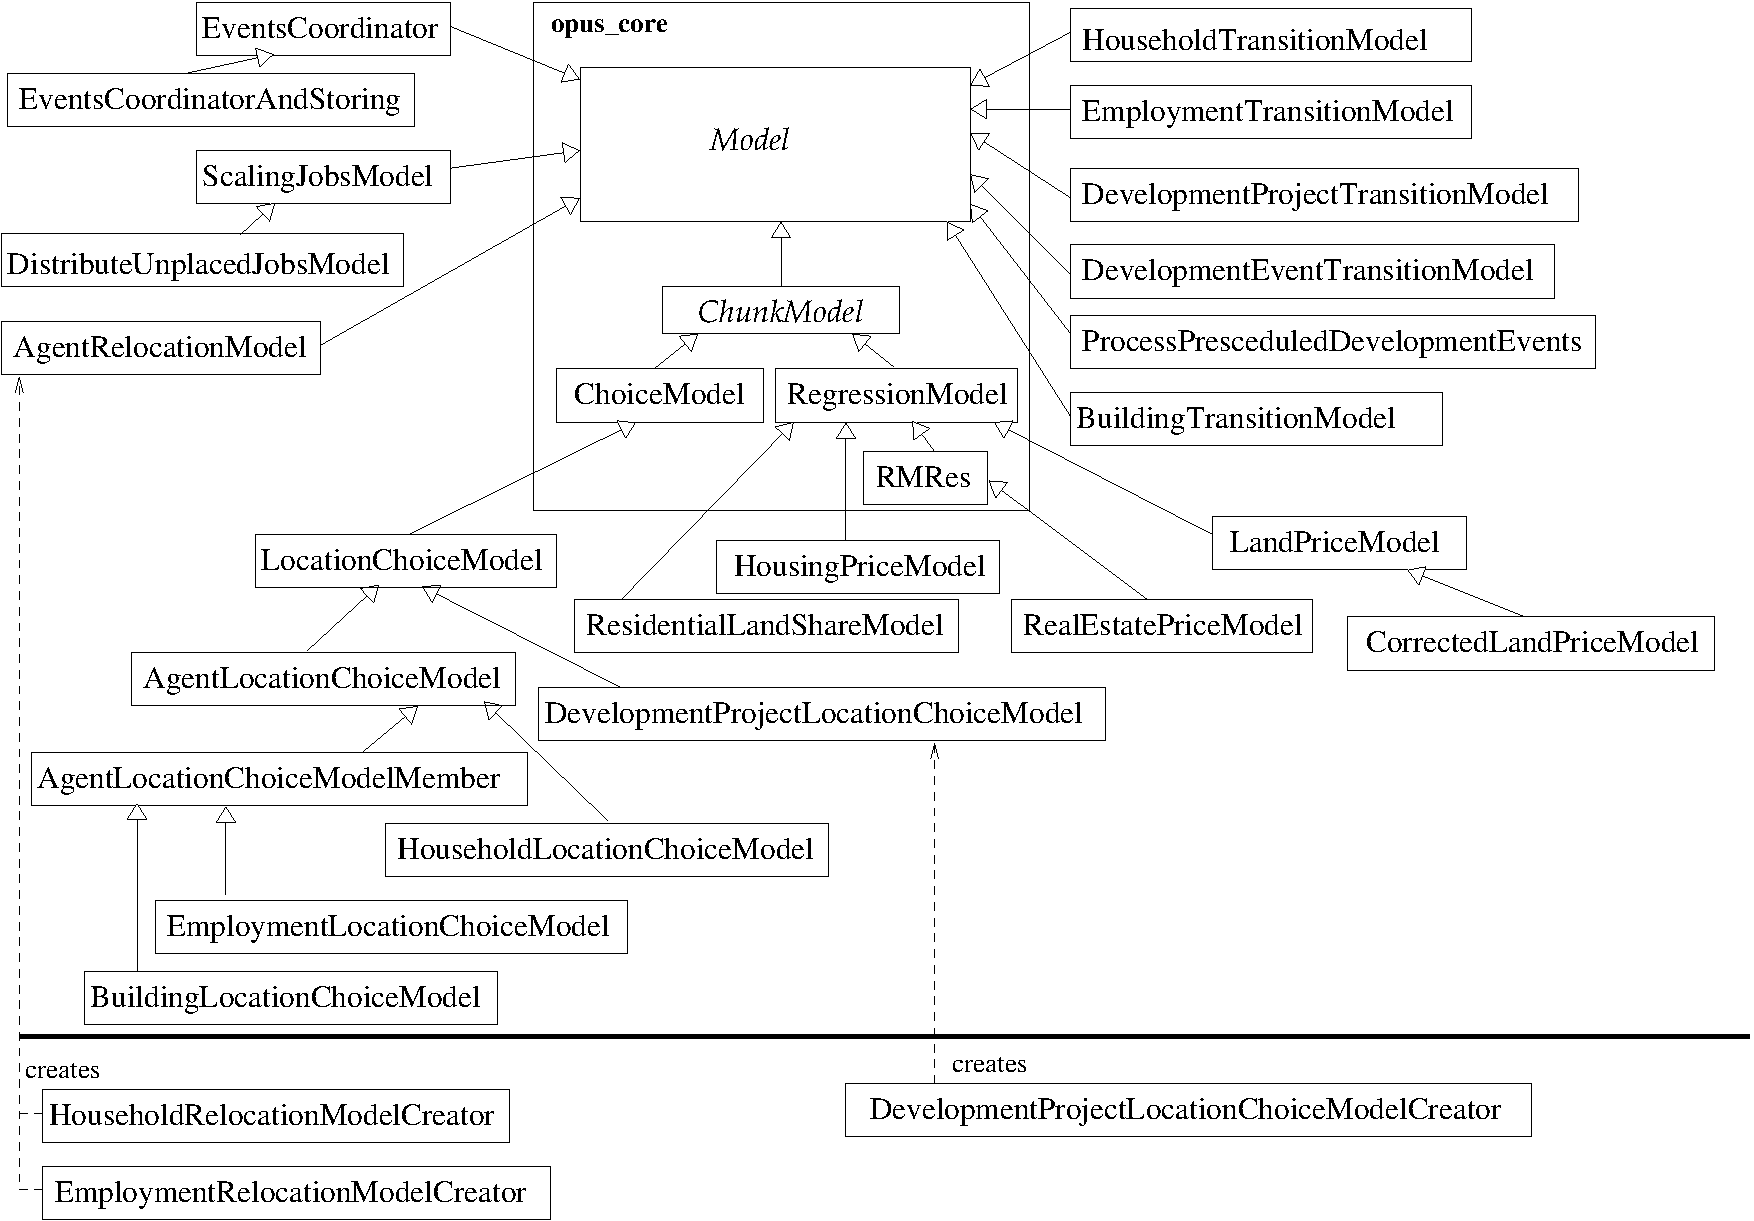
\includegraphics[scale=0.5]{images/urbansimmodels.pdf}
%end{latexonly}
\caption{\label{fig:urbansim-model}\small Models in \package{urbansim}. Solid arrows indicate the inheritance hierarchy:
$a \rightarrow b$ means $a$ inherits from $b$. Dashed arrows show relations between creators and models ($a$ creates $b$).}
\htmlonly{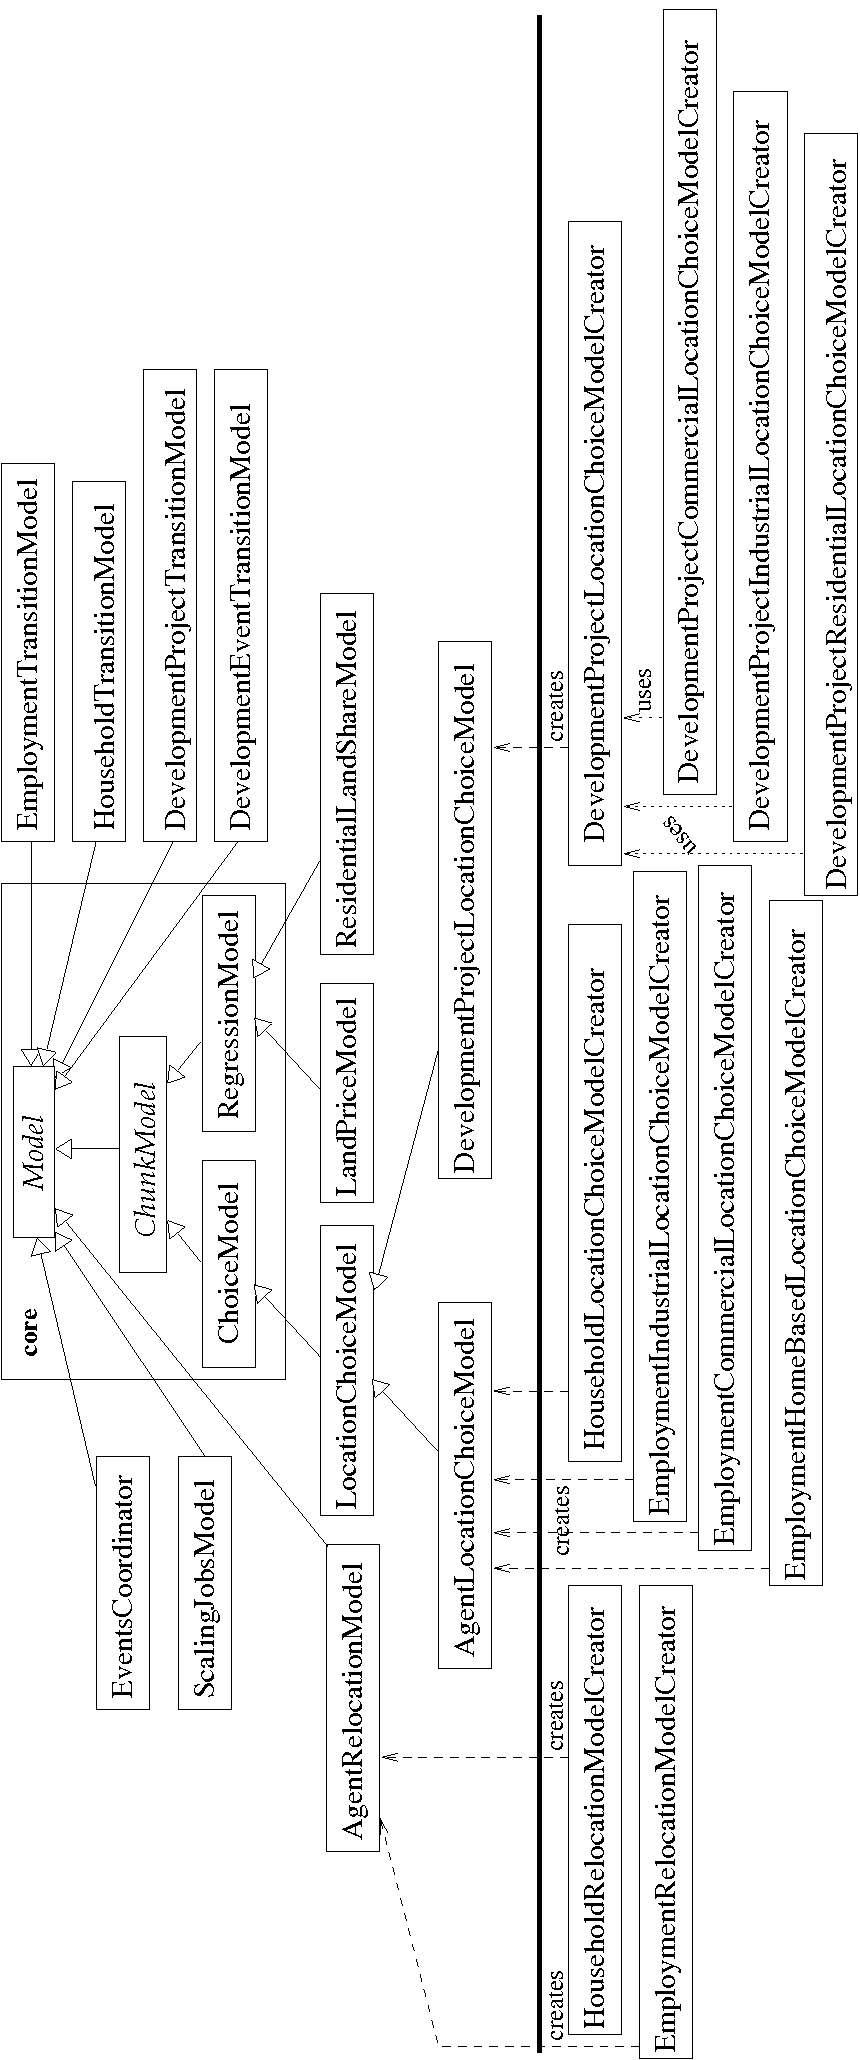
\includegraphics[scale=0.8]{images/urbansimmodels.jpg}}
\end{center}
\end{figure}

The models to execute when running UrbanSim are determined by the configuration
(see Section~\ref{sec:model-system-configuration}). Its entry ``models''  is a
list of character strings that identify the models to run in that order (see for example 
the list of models for running the gridcell version of UrbanSim on page~\pageref{pg:config-models}).
As discussed in Section~\ref{sec:model-controller-configuration}, 
the controller of each model points to one of the model classes shown in Figure~\ref{fig:urbansim-model}
and configures their inputs and outputs. In the following sections we describe each of the model classes in detail. 


\subsection{Land Price Model and Corrected Land Price Model}
\label{sec:land-price-model} 
\index{Land Price Model}\index{models!urbansim models!land price model}
%
The \class{LandPriceModel} \index{LandPriceModel@\class{LandPriceModel} class} 
predicts prices of land, in particular the
residential and non-residential land value for each member of the given
location set. The prediction is done via a regression procedure and thus,
the model is a child of the \class{RegressionModel} \index{RegressionModel@\class{RegressionModel} class} described in
Section~\ref{sec:regression-model}.

\subsubsection{Initialization}
%
The class is initialized by passing the following arguments:
\begin{description}
\item[regression_procedure] - a fully qualified name of the module/class in
  which the regression is implemented (see
  Section~\ref{sec:regression}). Default value is
  ``opus_core.linear_regression''.
\item[filter] - name of a variable/attribute used to filter out elements for
  the regression (applied to both, the \method{run()} and \method{estimate()}
  method). Default value is
  ``urbansim.gridcell.is_in_development_type_group_developable'' which requires an entry 'developable'
  in the table ``development_type_groups''. %(\ref{sec:development-tables-type-groups})
  It also requires that the location set is a gridcell set.
\item[submodel_string] - If model contains submodels, this character string
  specifies what attribute of the observation set determines those
  submodels. Default value is ``development_type_id''.
\item[run_config] - A collection of additional arguments that control a
  simulation run. It should be a python dictionary or of class \class{Resources}. Default is None.
\item[estimate_config] - A collection of additional arguments that control an
  estimation run. It should be a python dictionary or of class \class{Resources}. Default is None.
  \item[dataset_pool] - A pool of datasets needed for computation of variables. Default is None.
\end{description}
The constructor sets \verb|filter| as a class attribute and calls the parent
constructor (see Initialization in Section~\ref{sec:regression-model}).

\subsubsection{The Run Method}
%
{\it Input}:\\[1mm]
The \method{run()} method takes exactly the same arguments as its parent
class:\\
{\bf specification}, {\bf coefficients}, {\bf dataset}, {\bf index}, {\bf
  chunk_specification}, {\bf data_objects}, and {\bf run_config}.

{\it Algorithm}:\\[1mm]
If \verb|filter| is given in the initialization, \verb|index| is
updated to only those elements for which the value of
attribute/variable \verb|filter| is
larger than zero. It then invokes the \method{run()} method of
\class{RegressionModel} passing all arguments where
\verb|index| is possibly modified. The returned value of this call
is considered to be the prediction of the natural logarithm of total
land value for each element of \verb|dataset| included in
\verb|index|. Each of those values is then exponentiated and split
into residential and non-residential land value, using the attribute
``fraction_residential_land'' (this must be a known
attribute of \verb|dataset|).
Attributes ``residential_land_value'' and
``nonresidential_land_value'' (which also are expected to be known
attributes  of the \verb|dataset|) are modified by
replacing current values with the computed values.

If any of the computed values exceeds the maximal value of float32, a warning
is issued and the value is clipped to the maximal possible value.

{\it Output}:\\[1mm]
The method returns an index of values within \verb|dataset| for which the land
value was modified.

\subsubsection{The Estimate Method}
{\it Input}:\\[1mm]
The \method{estimate()} method takes exactly the same arguments as its parent
class: \\
{\bf specification}, {\bf dataset}, {\bf outcome_attribute}, {\bf index}, {\bf
  procedure}, {\bf data_objects}, and {\bf estimate_config}. The default value 
for \verb|outcome_attribute| is ``urbansim.gridcell.ln_total_land_value''.

{\it Algorithm}:\\[1mm]
The method applies the \verb|filter| (if given) in the same way as the
\method{run()} method. It then calls the parent method \method{estimate()}
passing all arguments and the possible modified \verb|index|.

{\it Output}:\\[1mm]
The method returns results of \method{estimate()} method of
\class{RegressionModel} (see Section~\ref{sec:regression-model}).

\subsubsection{Model Configuration}
%
This model is only used in the gridcell version of UrbanSim.
For a production run the model is
initialized with default values of the model 
constructor. The \method{run()} method is called by passing the
following arguments:
\begin{description}
\item[specification] - An
\class{EquationSpecification} object created with data from table
``land_price_model_specification''. 
\item[coefficients] - A \class{Coefficients} object created
with data from table ``land_price_model_coefficients''.
\item[dataset] - An instance of class \class{GridcellDataset} created with data
  from table ``gridcells'' (see Section~\ref{sec:gridcell-tables} for the
  table structure).
\item[index] - None. Thus, the model runs on all members of \verb|dataset| which are possibly 
filtered using a filter passed to the constructor (by default ``urbansim.gridcell.is_in_development_type_group_developable'', see
the Initialization paragraph).
\end{description}

\subsubsection{Corrected Land Price Model}
\index{Corrected Land Price Model}\index{CorrectedLandPriceModel@\class{CorrectedLandPriceModel} class}
%
This child model of \class{LandPriceModel} \index{LandPriceModel@\class{LandPriceModel} class} makes a
correction of the land value to avoid its declination with development type
change.

The \method{run()} method expects an additional argument, \verb|n_simulated_years|,
which gives the number of years that have been already simulated. If it is larger than 1,
after running its parent's code, a model called \class{CorrectLandValue} 
\index{CorrectLandValue@\class{CorrectLandValue} class}
is invoked. 
This model determines those members of \verb|dataset| whose
development type changed and at the same time have lower total land value when
comparing to previous simulated year. Values of the attributes 
``residential_land_value'' and ``nonresidential_land_value'' of these members
are replaced by values of the same attributes from previous year.

%
\subsection{Residential Land Share Model}
%
\label{sec:residential-land-share-model}
\index{Residential Land Share Model}\index{ResidentialLandShareModel@\class{ResidentialLandShareModel} class}
\index{models!urbansim models!residential land share model}

Residential land share model (implemented in class
\class{ResidentialLandShareModel}) predicts what fraction of each location is
residential land. It is a \class{RegressionModel} 
(Section~\ref{sec:regression-model}) with an only method overwritten, the
\method{run()} method.

\subsubsection{The Run Method}
%
{\it Input}:\\[1mm]
It takes the same arguments as the \method{run()} of its parent: \\
{\bf specification}, {\bf coefficients}, {\bf dataset}, {\bf index}, {\bf
  chunk_specification}, {\bf data_objects}, and {\bf run_config}.

{\it Algorithm}:\\[1mm]
The \method{run()} method of \class{RegressionModel} is invoked in order to
obtain a regression outcome $y$. If the run
was successful, the resulting quantity of this model, $y'$, is computed as
\[
y' = \frac{e^y}{1+e^y}
\]
$y'$ is an array of values for each member of \verb|dataset|  given by
\verb|index|. Those values are stored in the attribute  given by the class
property \verb|attribute_to_modify|. This is by default
``fraction_residential_land''. If such attribute does not exists in the
\verb|dataset|, it is created.

{\it Output}:\\[1mm]
The method returns $y'$.

\subsubsection{Model Configuration}
%
The model is used in the gridcell version of UrbanSim only.
It is called after the Events Coordinator (see Section~\ref{sec:events-coordinator}). 
It processes only those locations 
that were updated by the Events Coordinator.  The following
arguments are passed to the run:
\begin{description}
\item[specification] -  An
\class{EquationSpecification} object created with data from table
``residential_land_share_model_specification''. 
\item[coefficients] - A \class{Coefficients} object created
with data from table ``residential_land_share_model_coefficients''.
\item[dataset] - An instance of class \class{GridcellDataset} that was passed to
  the Events Coordinator.
\item[index] - Indices of the gridcells that were changed by the Events
  Coordinator, i.e. the first element of its output tuple.
\end{description}
 
%
\subsection{Housing Price Model}
%
\label{sec:housing-price-model}
\index{Housing Price Model}\index{models!urbansim models!housing price model}

The \class{HousingPriceModel} \index{HousingPriceModel@\class{HousingPriceModel} class} 
class predicts housing prices via a regression procedure and thus,
the model is a child of the \class{RegressionModel} \index{RegressionModel@\class{RegressionModel} class} described in
Section~\ref{sec:regression-model}.

\subsubsection{Initialization}
%
The class is initialized by passing the following arguments:
\begin{description}
\item[regression_procedure] - a fully qualified name of the module/class in
  which the regression is implemented (see
  Section~\ref{sec:regression}). Default value is
  ``opus_core.linear_regression''.
\item[filter_attribute] - name of a variable/attribute used to filter out elements for
  the regression (applied to both, the \method{run()} and \method{estimate()}
  method). Default value is
  ``urbansim.gridcell.has_residential_units'' which requires an entry 'residential_units'
  in the ``gridcells'' table.
  It also requires that the regression is done on a gridcell dataset.
\item[submodel_string] - If model contains submodels, this character string
  specifies what attribute of the observation set determines those
  submodels. Default value is ``development_type_id''.
\item[run_config] - A collection of additional arguments that control a
  simulation run. It should be a python dictionary or of class \class{Resources}. Default is None.
\item[estimate_config] - A collection of additional arguments that control an
  estimation run. It should be a python dictionary or of class \class{Resources}. Default is None.
  \item[dataset_pool] - A pool of datasets needed for computation of variables. Default is None.
\end{description}
The constructor sets \verb|filter_attribute| as a class attribute and calls the parent
constructor (see Initialization in Section~\ref{sec:regression-model}).

\subsubsection{The Run Method}
%
{\it Input}:\\[1mm]
The \method{run()} method takes exactly the same arguments as its parent
class:\\
{\bf specification}, {\bf coefficients}, {\bf dataset}, {\bf index}, {\bf
  chunk_specification}, {\bf data_objects}, and {\bf run_config}.

{\it Algorithm}:\\[1mm]
If \verb|filter_attribute| is given in the initialization, \verb|index| is
updated to only those elements for which the value of
attribute/variable \verb|filter_attribute| is
larger than zero. It then invokes the \method{run()} method of
\class{RegressionModel} passing all arguments where
\verb|index| is possibly modified. The returned value of this call
is considered to be the prediction of housing price. \verb|dataset| is expected to have 
an attribute 'housing_price' which is modified for members given by \verb|index| by the computed values.

{\it Output}:\\[1mm]
The method returns None.

\subsubsection{The Estimate Method}
{\it Input}:\\[1mm]
The \method{estimate()} method takes exactly the same arguments as its parent
class: \\
{\bf specification}, {\bf dataset}, {\bf outcome_attribute}, {\bf index}, {\bf
  procedure}, {\bf data_objects}, and {\bf estimate_config}. The default value 
for \verb|outcome_attribute| is ``housing_price''.

{\it Algorithm}:\\[1mm]
The method applies the \verb|filter_attribute| (if given) in the same way as the
\method{run()} method. It then calls the parent method \method{estimate()}
passing all arguments and the possible modified \verb|index|.

{\it Output}:\\[1mm]
The method returns results of \method{estimate()} method of
\class{RegressionModel} (see Section~\ref{sec:regression-model}).

%
\subsection{Real Estate Price Model}
%
\label{sec:real-estate-price-model}
\index{Real Estate Price Model}\index{models!urbansim models!real estate price model}

The \class{RealEstatePriceModel} \index{RealEstatePriceModel@\class{RealEstatePriceModel} class}
class predicts real estate prices via a regression procedure (see Section~\ref{sec:model-system-real-estate-price-model}).
In order to avoid jumps in prices for the first simulated year, the initial residuals are 
added to the regression outcomes. Thus,
the model is a child of the \class{RegressionModelWithInitialResiduals}  
\index{RegressionModelWithInitialResiduals@\class{RegressionModelWithInitialResiduals} class}
described in
Section~\ref{sec:regression-model} in a paragraph on page~\pageref{page:regression-model-with-initial-residuals}.

\subsubsection{Initialization}
%
The class is initialized by passing the following arguments:
\begin{description}
\item[regression_procedure] - a fully qualified name of the module/class in
  which the regression is implemented (see
  Section~\ref{sec:regression}). Default value is
  ``opus_core.linear_regression''.
\item[filter_attribute] - name of a variable/attribute used to filter out elements for
  the regression (applied to both, the \method{run()} and \method{estimate()}
  method). Default value is None.
\item[submodel_string] - If model contains submodels, this character string
  specifies what attribute of the observation set determines those
  submodels. Default value is ``building_type_id''.
\item[outcome_attribute] - A required attribute of the observation dataset. It is used to compute the 
initial residuals. Default is 'unit_price'. The attribute should be a primary attribute, unless 
it starts with the string 'ln_'. In such a case the observation set is required to have an attribute 
matching the \verb|outcome_attribute| without the prefix 'ln_'. 
\item[run_config] - A collection of additional arguments that control a
  simulation run. It should be a python dictionary or of class \class{Resources}. Default is None.
\item[estimate_config] - A collection of additional arguments that control an
  estimation run. It should be a python dictionary or of class \class{Resources}. Default is None.
  \item[dataset_pool] - A pool of datasets needed for computation of variables. Default is None.
\end{description}
The constructor sets \verb|filter_attribute| as a class attribute and calls the parent
constructor (see Initialization in Section~\ref{sec:regression-model}).

\subsubsection{The Run Method}
%
{\it Input}:\\[1mm]
The \method{run()} method takes exactly the same arguments as its parent
class:\\
{\bf specification}, {\bf coefficients}, {\bf dataset}, {\bf index}, {\bf
  chunk_specification}, {\bf data_objects}, and {\bf run_config}.

{\it Algorithm}:\\[1mm]
If \verb|filter_attribute| is given in the initialization, \verb|index| is
updated to only those elements for which the value of
attribute/variable \verb|filter_attribute| is
larger than zero. It then invokes the \method{run()} method of
\class{RegressionModel} passing all arguments where
\verb|index| is possibly modified. The returned value of this call
is considered to be the prediction for the given \verb|outcome_attribute|.
If \verb|outcome_attribute| starts with 'ln_', the values are exponentiated 
and stored as a \verb|dataset| attribute of the same name but without the prefix 'ln_'.
Otherwise the values of \verb|outcome_attribute| are overwritten by the new values. 
Only values are overwritten that correspond to dataset members given by index.

{\it Output}:\\[1mm]
The predicted values stored in the \verb|dataset| are returned. 

\subsubsection{The Estimate Method}
{\it Input}:\\[1mm]
The \method{estimate()} method takes exactly the same arguments as its parent
class: \\
{\bf specification}, {\bf dataset}, {\bf outcome_attribute}, {\bf index}, {\bf
  procedure}, {\bf data_objects}, and {\bf estimate_config}. The default value 
for \verb|outcome_attribute| is ``unit_price''.

{\it Algorithm}:\\[1mm]
The method applies the \verb|filter_attribute| (if given) in the same way as the
\method{run()} method. It then calls the parent method \method{estimate()}
passing all arguments and the possible modified \verb|index|.

{\it Output}:\\[1mm]
The method returns results of \method{estimate()} method of
\class{RegressionModel} (see Section~\ref{sec:regression-model}).

\subsubsection{Model Configuration}
%
In the {\bf parcel} version of UrbanSim, the model is initialized as follows:
\begin{description}
\item[submodel_string] - 'land_use_type_id'
\item[outcome_attribute] - 'ln_unit_price=ln(urbansim_parcel.parcel.unit_price)'
\item[filter_attribute] - 'numpy.logical_or(urbansim_parcel.parcel.building_sqft, urbansim_parcel.parcel.is_land_use_type_vacant)'
\end{description}

In the {\bf zone} version of UrbanSim, the model is initialized as follows:
\begin{description}
\item[submodel_string] - 'building_type_id'
\item[outcome_attribute] - 'ln_unit_price=ln(pseudo_building.avg_value)'
\end{description}
Remaining arguments in both cases get the default values of the model 
constructor.

The \method{run()} method is called by passing the
following arguments:
\begin{description}
\item[specification] - An
\class{EquationSpecification} object created with data from table
``real_estate_price_model_specification''. 
\item[coefficients] - A \class{Coefficients} object created
with data from table ``real_estate_price_model_coefficients''.
\item[dataset] - For parcel projects, this is an instance of class \class{ParcelDataset} created with data
  from table ``parcels''. For zone projects, this is an instance of class \class{PseudoBuildingDataset}.
\item[index] - None. Thus, the model runs on all members of \verb|dataset| which are in case of the parcel project 
filtered using the filter passed to the constructor.
\item[run_config] - For zone projects it is None. For parcel projects it has entries:
\begin{verbatim}
{
  'exclude_outliers_from_initial_error': True, 
  'outlier_is_less_than': 3, 
  'outlier_is_greater_than': 7
}
\end{verbatim}
\end{description}
%

\subsection{Location Choice Model}
%
\label{sec:location-choice-model}
\index{Location Choice Model} \index{models!urbansim models!location choice model}
\index{LocationChoiceModel@\class{LocationChoiceModel} class}

A location choice model is a choice model where the set of alternatives is a
set of locations.

The class \class{LocationChoiceModel} is a child of \class{ChoiceModel} \index{ChoiceModel@\class{ChoiceModel} class}
described in Section~\ref{sec:choice-model}. In addition, it allows sampling
of alternatives and filtering alternatives according to a specified filter.

\subsubsection{Initialization}
%
The class is initialized by passing the following arguments:
\begin{description}
\item[location_set] - A dataset of locations to be chosen from.
\item[sampler] - A fully qualified name of the module for sampling
  alternatives. Default value is ``opus_core.samplers.weighted_sampler''. If
  this argument is set to None, no sampling is performed.
\item[utilities] - A fully qualified name of the module for computing utilities
  (see Section~\ref{sec:utilities}). Default value is
  ``opus_core.linear_utilities''.
\item[probabilities] - A fully qualified name of the module for computing
  probabilities (see Section~\ref{sec:probabilities}). Default value is
  ``opus_core.mnl_probabilities''.
\item[choices] - A fully qualified name of the module for determining
  final choices (see Section~\ref{sec:choices}). Default value is
  ``opus_core.random_choices''.
\item[interaction_pkg] - This argument is only relevant if there is an
  explicit implementation of an interaction dataset that corresponds to
  interaction between agents and choices (such as those from
  Table~\ref{tab:urbansim-interaction-datasets}). It then determines the
  package in which the module lives. Default value is
  ``urbansim.datasets''. 
\item[filter] - It is either a string specifying an attribute name of the
  filter for filtering out locations to be chosen from, or a 1D/2D array giving the filter directly, or a dictionary
  specifying filter for each submodel. If it is None (default), no filter is
  applied.
\item[submodel_string] - If model contains submodels, this character string
  specifies what agent's attribute determines those submodels. If it is None
  (default), no division into submodels is applied.
\item[location_id_string] - A character string giving the fully qualified name of an agent attribute
  that specifies the location. It is only needed when the attribute is a variable (i.e. not a primary attribute).
  Default is None.
\item[run_config] - A collection of additional arguments that control a
  simulation run. It should be of class \class{Resources}. Default is None.
\item[estimate_config] - A collection of additional arguments that control an
  estimation run. It should be of class \class{Resources}. Default is None.
\item[dataset_pool] - A pool of datasets needed for computation of variables. Default is None.
\end{description}
The method calls the constructor of its parent class. Then, it creates a
\class{Sampler} object from the argument \verb|sampler| using
\class{SamplerFactory}. It sets value of the argument \verb|filter| as a class
property \verb|filter|.

%
\subsubsection{The Run Method}
%
The \method{run()} method runs the simulation of location choice model on basis
of a given specification and coefficients.

{\it Input}:\\[1mm]
It takes the same arguments as the \method{run()} method of its parent (see
Section~\ref{sec:choice-model} for more details): \\
{\bf specification}, {\bf coefficients}, {\bf agent_set}, {\bf agents_index},
{\bf chunk_specification}, {\bf data_objects}, and {\bf run_config}.

{\it Algorithm}:\\[1mm]
The model is processed in chunks. The \method{run_chunk()} method moves
the agents out of their locations, i.e. the values of an
\verb|agent_set| attribute of the same name as the unique identifier of
\verb|location_set| is set to $-1$ for each agent of the currently processed
chunk. If \verb|agent_set| does not have this attribute, it is appended to it.

If an entry ``compute_capacity_flag'' is given in \verb|run_config| and its
value is True, an entry ``capacity_string'' is expected in \verb|run_config|
which gives the name of attribute/variable of \verb|location_set| that
determines capacity for each location. In such a case, after removing agents
from their locations, the capacity is computed using method
\method{determine_units_capacity()}. Note that by removing agents of only the
current chunk from their locations, the capacity is influenced by only those
agents. Each chunk then see the state of the world updated by all previously
running chunks.

By default, the capacity values are used as weights of locations in the case of sampling.
This can be changed by setting the entry 'weights_for_simulation_string' of \verb|run_config|, 
which should be a fully-qualified variable name of the location set that determines weights. 
The weights are multiplied by the filter given in the initialization.  The
model then invokes sampling of alternatives by calling the
\method{run()} method of the sampler class, passing the possibly filtered
weights. The parent class then takes care of creating the interaction set, for
agents of the corresponding chunk and possibly sampled alternatives and of
running the \verb|upc_sequence|. 

The location IDs that agents chose in the choice process are stored
in the \verb|agent_set| attribute specifying locations.

{\it Output}:\\[1mm]
The method returns an array of size \verb|agents_index|,
representing the location IDs that agents (elements of
\verb|agent_set| determined by \verb|agents_index|) made. Agents
whose choice is less equal zero were not included in the choice
process, for example because they do not belong to any submodels
given in the specification.


\subsubsection{The Estimate Method}
%
{\it Input}:~\\[1mm]
The \method{estimate()} method takes the same arguments as its parent class:\\
{\bf specification}, {\bf agent_set}, {\bf agents_index}, {\bf procedure},
{\bf data_objects}, and {\bf estimate_config}.

{\it Algorithm}:\\[1mm]
As in the \method{run()} method, if ``compute_capacity_flag'' is given in
\verb|estimate_config| and its value is True, an entry ``capacity_string'' is
expected in \verb|estimate_config| which gives the name of attribute/variable 
of \verb|location_set| that determines capacity for each location. In such a
case, the capacity is computed using method
\method{determine_units_capacity_for_estimation()}.

The weights for sampling alternatives are determined by an optional entry
``weights_for_estimation_string'' in \verb|estimate_config| which should be an
attribute/variable name of \verb|location_set|. They are multiplied by the
given \verb|filter| (if any) and as in the case of the \method{run()} method,
sampling is performed using those weights. The parent class performs then the
estimation.

{\it Output}:\\[1mm]
The method passes the return values of its parent method \method{estimate()},
i.e. a tuple of the created \class{Coefficient} object and a
dictionary with entries for each submodel equals a dictionary returned by the
\verb|run()| method of \verb|procedure| for that submodel.

%
\subsubsection{Model Configuration}
%
The arguments \verb|run_config| and \verb|estimate_config| are collections of
parameters that control the \method{run()} and \method{estimate()} method,
respectively. In addition to the mentioned entries ``compute_capacity_flag'',
``capacity_string'', ``weights_for_simulation_string'', and ``weights_for_estimation_string'', they can contain entries
``sample_proportion_locations'' and ``sample_size_locations''. Both entries
control the size of sampled alternatives, the first one as a relative number,
the latter one as an absolute number. The latter one has a priority over the
first one.

\verb|estimate_config| can also contain an entry 'chunk_specification_for_estimation',
which should be an object of class \class{ChunkSpecification} (see Section~\ref{sec:resources}).
It controls the number of chunks in which the sampling is done for the estimation.

%
%
\subsection{Development Project Location Choice Model}
%
\label{sec:development-project-lcm}
\index{Development Project Location Choice Model} \index{models!urbansim models!development project location choice model}
\index{DevelopmentProjectLocationChoiceModel@\class{DevelopmentProjectLocationChoiceModel} class}
%
The Development project location choice model implemented in the
\package{urbansim} package simulates a process where
development projects of a specific type choose locations to be placed into (see Section~\ref{real-estate-development-model}
on page~\pageref{real-estate-development-model-gridcell}).
The class \class{DevelopmentProjectLocationChoiceModel} is a child of
\class{LocationChoiceModel} \index{LocationChoiceModel@\class{LocationChoiceModel} class} described in
Section~\ref{sec:location-choice-model}.

\subsubsection{Initialization}
%
The class is initialized by passing the following arguments:
\begin{description}
\item[location_set] - A dataset of locations to be chosen from.
\item[project_type] - A character string determining the type of the projects
  for this model, such as 'commercial' or 'residential'. 
\item[units] - A character string giving the name of the attribute that
  determines sizes of projects.
\item[developable_maximum_unit_variable_full_name] -  A character string determining
  which Opus variable of the location set to use for computing the maximum developable units
  in each location.
\item[developable_minimum_unit_variable_full_name] -  A character string determining
  which Opus variable of the location set to use for computing the minimum developable units
  in each location. Default is None which means there is no restriction on the minimum number of units.
\item[model_name] - An optional argument giving the model name. Default is None.
\item[...] all remaining arguments from the constructor of
  \class{LocationChoiceModel}. 
\end{description}

The arguments are set as class properties and the parent constructor is invoked.

\subsubsection{The Run Method}
%
{\it Input}:\\[1mm]
It takes the same arguments as the \method{run()} method of its parent: \\
{\bf specification}, {\bf coefficients}, {\bf agent_set}, {\bf agents_index},
{\bf chunk_specification}, {\bf data_objects}, and {\bf run_config}.

The \verb|agent_set| is expected to be an instance of
\class{DevelopmentProjectDataset}. It is assumed that initially all projects are
unplaced.

{\it Algorithm}:\\[1mm]
The model must be set to use capacity (via entries ``compute_capacity_flag''
and ``capacity_string'' in \verb|run_config|).  The capacity attribute is
considered as a variable that is 1 for locations that are developable for this
particular project type, otherwise 0. This means that no more than one project
of the same type can occupy one location. The method
\method{determine_units_capacity()} assures that locations taken in previous
chunks are marked as taken.

The weight array for sampling is constructed in each chunk by combining
information about project sizes and minimum and maximum developable units in
each location.  Thus, the weight array is a 2-d array which implies that
different projects have different weights for the same locations, depending on
their size. The dimension of the location axis of this array is for memory
reasons reduced to only locations that are developable. No additional
filtering is done (the model sets the class property \verb|filter| to
\verb|None|).

The class overwrites its parent's method \verb|get_agents_order()| in a way that it
sorts the agents according to their sizes in descending order. This means that
larger projects enter the choice process first.

The \method{run()} method proceeds otherwise as defined in the parent class.

{\it Output}:~\\[1mm]
It returns results of its parent class.

\subsubsection{The Estimate Method}
%
The \method{estimate()} method is identical to its parent method
\method{estimate()}.


\subsubsection{Creators}
%
The model can be created using a pre-defined creator in \package{urbansim}.
The class\\
\class{DevelopmentProjectLocationChoiceModelCreator}\index{DevelopmentProjectLocationChoiceModelCreator@\class{DevelopmentProjectLocationChoice\-Model\-Creator} class} 
sets useful default
values for arguments of the constructor. The model is by default initialized with:
\begin{description}
\item[sampler] - ``opus_core.samplers.weighted_sampler''
\item[utilities] - ``opus_core.linear_utilities''
\item[probabilities] - ``opus_core.mnl_probabilities''
\item[choices] - ``urbansim.first_agent_first_choices'' (see
  Section~\ref{sec:urbansim-choices})
\item[submodel_string] - ``size_capacity''
\item[filter] - \verb|''urbansim.gridcell.developable_%s'' % units|
% \item[units] - `` '' (empty string)
\item[residential] - False, project type is not of residential type
\end{description}
Entries of \verb|run_config| are set as to:
\begin{verbatim}
{   "compute_capacity_flag": True,
    "sample_size_locations": 30,
    "capacity_string": "urbansim.gridcell.is_developable_for_%s" % units }
\end{verbatim}
The variable \verb|units| in the last line is taken from a model configuration
that is passed to the creator in an entry ``units'' of the corresponding
project type (see model configuration on
page~\pageref{page:model-configuration}).

Entries of \verb|estimate_config| are set as to:
\begin{verbatim}
{   "estimation": "opus_core.bhhh_mnl_estimation",
    "sample_size_locations": 30,
    "estimation_size_agents": 1.0  }
\end{verbatim}


\subsubsection{Model Configuration}
%
This implementation is used only in the gridcell version of UrbanSim.
The production run is configured with three development project
types: ``residential'', ``commercial'', and ``industrial''. Thus, there are
three instances of the model, each initialized with the particular project
type and a \class{GridcellDataset} as \verb|location_set|.  Each of the models 
runs only if the Development Project Transition Model returns some projects
for the project type, i.e. the output value for this particular project type
is not None.  The \method{run()} method of each of the model is called by
passing the following arguments:
\begin{description}
\item[specification] - An
\class{EquationSpecification} object created with data from table
``\%s_development_location_choice_model_specification''. 
\item[coefficients] - A \class{Coefficients} object created
with data from table ``\%s_development_location_choice_model_coefficients''. 
\item[agent_set] - A \class{DevelopmentProjectDataset} returned by the Development
  Project Transition Model in its entry for this particular project type.
\end{description}
The ``\%s'' in the above character strings are replaced by project type.

By default the model runs on submodels determined by the sizes of the projects. Specifically,
the initialization method is called with the argument \verb|submodel_string=urbansim.development_project.size_category|
(see \ref{sec:DPTM-configuration} for the definition of the categories). Note that $n$ numbers in
the categories list correspond to $n+1$ submodels. For running the model on all projects without categorizing, 
set the \verb|sub_model_id| field of the specification and coefficients table to $-2$.

%
%
\subsection{Agent Location Choice Model}
%
\label{sec:agent-lcm}
\index{Agent Location Choice Model}\index{models!urbansim models!agent location choice model}
\index{AgentLocationChoiceModel@\class{AgentLocationChoiceModel} class}

The class \class{AgentLocationChoiceModel} is a child
of \class{LocationChoiceModel}\index{LocationChoiceModel@\class{LocationChoiceModel} class} described in
Section~\ref{sec:location-choice-model}. It can deal with exceeded capacity of locations.

\subsubsection{Initialization}
%
In addition to its parents' arguments {\bf location_set}, {\bf sampler}, {\bf utilities}, {\bf probabilities}, 
{\bf choices}, {\bf interaction_pkg}, {\bf filter}, {\bf submodel_string}, {\bf location_id_string}, 
{\bf run_config}, {\bf estimate_config}, and {\bf dataset_pool}, it takes arguments:
\begin{description}
\item[model_name] - character string giving the name of the model.
\item[short_name] - character string giving an abreviation of the model name which is used 
only by the model logger.
\item[variable_package] - Opus package used for computing variables/expressions given in \verb|run_config|
end \verb|estimate_config|. Default is 'urbansim'.
\end{description}

The constructor completes any unqualified variable names given in 
arguments, \verb|run_config| and \verb|estimate_config| to fully-qualified
names, by using the dataset name of the given \verb|location_set| and  \verb|variable_package|.
Then the parent constructor is called.

\subsubsection{The Run Method}
%
{\it Input:}\\[1mm]
In addition to its parents' arguments {\bf specification}, {\bf coefficients}, {\bf agent_set}, {\bf agents_index},
{\bf chunk_specification}, {\bf data_objects}, and {\bf run_config}, it accepts:
\begin{description}
\item[maximum_runs] - maximum number of iterations (see the algorithm below). Default is 10.
\end{description}
The method puts the parent method
\method{run()} into a loop which is repeated whenever there is an
overflow in the capacity after the last run. This behavior is
activated only if the ``compute_capacity_flag'' entry of
\verb|run_config| is set to True. In such a case, \verb|run_config|
also should have entries ``number_of_units_string'' giving the
variable name for computing number of available
units in each location, and ``number_of_agents_string'' giving the
variable name for computing the number of agents
located in each location. Those variables are
computed and the difference in their values determines the
overfilled locations. If there are any such locations, an
appropriate number of agents (from the set given by
\verb|agents_index|) are removed from their locations and the parent
\method{run()} method is called again. The number of such iterations is
given by the argument \verb|maximum_runs|.

%
\subsection{Household Location Choice Model}
\index{Household Location Choice Model} \index{models!urbansim models!household location choice model}
%
This model (class \class{HouseholdLocationChoiceModel}) 
\index{HouseholdLocationChoiceModel@\class{HouseholdLocationChoiceModel} class}
is an Agent Location Choice Model \index{AgentLocationChoiceModel@\class{AgentLocationChoiceModel} class} that makes default settings
of various arguments usable in the context of households
choosing their locations. See also Section~\ref{sec:model-system-household-location-choice-model}.
The model is initiated with the arguments and their default values
listed below. They are either directly passed to the constructor of the parent or packed into 
the \verb|run_config| and/or
\verb|estimate_config| arguments under appropriate names.
\begin{description}
\item[location_set] - no default value
\item[sampler] - "opus_core.samplers.weighted_sampler"
\item[utilities] - "opus_core.linear_utilities" 
\item[choices] - "opus_core.random_choices"
\item[probabilities] - "opus_core.mnl_probabilities"
\item[estimation] - "opus_core.bhhh_mnl_estimation"
\item[capacity_string] - "vacant_residential_units"
\item[estimation_weight_string] - "residential_units" 
\item[simulation_weight_string] - None. If this argument is None, weights are proportional to the capacity.
\item[number_of_agents_string] - "number_of_households"
\item[number_of_units_string] - "residential_units"            
\item[sample_proportion_locations] - None
\item[sample_size_locations] - 30 
\item[estimation_size_agents] - 1.0 
\item[compute_capacity_flag] - True 
\item[filter] - None
\item[submodel_string] - None 
\item[location_id_string] - None
\item[demand_string] - None. If this argument is not None, the aggregated demand for locations 
  are stored in this attribute (see description of the \method{run} method in Section~\ref{sec:choice-model}).
\item[run_config] - None.
\item[estimate_config] - None
\item[dataset_pool] - None
\item[variable_package] - "urbansim"
\end{description}


\subsubsection{Model Configuration}
%
Our gridcell version of UrbanSim configures the Household Location Choice Model with a 
\class{GridcellDataset} passed as
argument {\bf location_set} of the constructor. The zone version uses here a \class{ZoneDataset} object
and the parcel version uses a \class{BuildingDataset}.
Additionally, in all versions the default
value of {\bf choices} is overwritten by ``urbansim.lottery_choices'' (see
Section~\ref{sec:urbansim-choices}).

The following arguments are passed to
  the \method{run()} method:
\begin{description}
\item[specification] - An \class{EquationSpecification} object created with
  data from table ``household_location_choice_model_specification''. 
\item[coefficients] - A \class{Coefficients} object created with data from
  table ``household_location_choice_model_coefficients''.
\item[agent_set] - A \class{HouseholdDataset} object used in Household Relocation
  Model.
\item[agents_index] - Results of Household Relocation Model (see page~\pageref{page:HRM}). 
\index{Household Relocation Model} 
Make sure that model is turned on 
when running Household Location Choice Model.
\end{description}


\subsection{Agent Location Choice Model Member}
%
\label{sec:agent-lcm-member}
\index{Agent Location Choice Model Member}
\index{AgentLocationChoiceModelMember@\class{AgentLocationChoiceModelMember} class}
%
This model is a child of \class{AgentLocationChoiceModel} \index{AgentLocationChoiceModel@\class{AgentLocationChoiceModel} class}
(Section~\ref{sec:agent-lcm}) that is used 
for running the parent class with different subsets of the agents.

\subsubsection{Initialization}
%
The class is initialized by passing the following arguments:
\begin{description}
\item[group_member] - An object of class \class{ModelGroupMember}\index{ModelGroupMember@\class{ModelGroupMember} class} (see Section~\ref{sec:model-group}) 
  determining for which member is this model initialized.
\item[location_set] - A dataset of locations.
\item[agents_grouping_attribute] - An attribute of the agent set that is used for classifying agents into the member groups. 
\end{description}
Other arguments of the parent class can be passed. 

\subsubsection{The Run and Estimate Methods}
%
For both methods, the agents that correspond to the given member are selected and the model is run/estimated only
on those agents. The return array of the \method{run()} method contains -1 for agents that do not belong to the group.

The \method{prepare_for_estimate} method appends the member name as prefix in front of the specification and coefficients tables.

\subsection{Employment Location Choice Model}
\label{sec:elcm} 
\index{Employment Location Choice Model}\index{models!urbansim models!employment location choice model}
%
The class \class{EmploymentLocationChoiceModel} \index{EmploymentLocationChoiceModel@\class{EmploymentLocationChoiceModel} class} 
is a child of \class{AgentLocationChoiceModelMember}. \index{model group}\index{AgentLocationChoiceModelMember@\class{AgentLocationChoiceModelMember} class}
Its default settings
of various arguments makes the model usable in the context of jobs choosing their locations. 
See also Section~\ref{sec:model-system-employment-location-choice-model}.
It is initialized by the following arguments and default values:
\begin{description}
\item[group_member] - no default value
\item[location_set] - no default value
\item[agents_grouping_attribute] - 'job.building_type'
\item[sampler] - "opus_core.samplers.weighted_sampler"
\item[utilities] - "opus_core.linear_utilities" 
\item[choices] - "opus_core.random_choices"
\item[probabilities] - "opus_core.mnl_probabilities"
\item[estimation] - "opus_core.bhhh_mnl_estimation"
\item[capacity_string] - "vacant_SSS_job_space"
\item[estimation_weight_string] - "total_number_of_possible_SSS_jobs"
\item[simulation_weight_string] - None. If this argument is None, weights are proportional to the capacity.
\item[number_of_agents_string] - "number_of_SSS_jobs"
\item[number_of_units_string] - "total_number_of_possible_SSS_jobs"          
\item[sample_proportion_locations] - None
\item[sample_size_locations] - 30 
\item[estimation_size_agents] - 1.0 
\item[compute_capacity_flag] - True 
\item[filter] - None
\item[submodel_string] - "sector_id"
\item[location_id_string] - None
\item[demand_string] - None. If this argument is not None, the aggregated demand for locations 
  are stored in this attribute (see description of the \method{run} method in Section~\ref{sec:choice-model}).
\item[run_config] - None.
\item[estimate_config] - None
\item[dataset_pool] - None
\item[variable_package] - "urbansim"
\end{description}
The initialization procedure replaces any occurence of the string 'SSS' in the various arguments
by the name of the group member. For example, if the group member corresponds to the 'commercial' building type of jobs,
the value of argument \verb|capacity_string| would be converted to "vacant_commercial_job_space".
Arguments are then either directly passed to the constructor of the parent or packed into 
the \verb|run_config| and/or
\verb|estimate_config| arguments under appropriate names.

\subsubsection{Model Configuration}
%
In the gridcell and zone version of UrbanSim, this model is called by default for members 'commercial', 
'industrial', and 'home_based'.
In the parcel version, we use only the group member 'non_home_based'. Note that 
these names must be contained in the table \file{job_building_types}. 

The following arguments are passed to the constructors of models for all members:
\begin{description}
\item[location_set] - A \class{GridcellDataset} object in the gridcell project, \class{ZoneDataset} in the zone project,
  and \class{BuildingDataset} in the parcel project.
\item[choices] - 'urbansim.lottery_choices'
\end{description}
The default submodel_string is `sector_id', which associates submodels with the employment sectors defined in the table \file{employment_sectors}.  
Additionally, the member 'home_based' overwrites the arguments {\bf estimation_weight_string} by the value 'residential_units' 
and {\bf number_of_units_string} by the value 'residential_units'.

In all versions, the \method{run()} method is called with the following arguments:
\begin{description}
\item[specification] - Uses data from
  ``\%s_employment_location_choice_model_specification'' where \%s is replaced by the member name.
\item[coefficients] - Uses data from ``\%s_employment_location_choice_model_coefficients'' 
    where \%s is replaced by the member name.
\item[agent_set] - A \class{JobDataset} object used in Employment Relocation Model.
\item[agents_index] - Results of Employment Relocation Model (see page~\pageref{page:ERM}).\index{Employment Relocation Model} 
Make sure that model is turned on 
when running Employment Location Choice Model.
\end{description}
 
%
\subsection{Building Location Choice Model}
\label{sec:BLCM}
\index{Building Location Choice Model}\index{models!urbansim models!building location choice model}
%
The class \class{BuildingLocationChoiceModel} \index{BuildingLocationChoiceModel@\class{BuildingLocationChoiceModel} class} 
is a child of \class{AgentLocationChoiceModelMember}. \index{model group}\index{AgentLocationChoiceModelMember@\class{AgentLocationChoiceModelMember} class}
Its default settings
of various arguments makes the model usable in the context of buildings choosing their locations.
It is an alternative model to the Development Project Location Choice Model \index{Development Project Location Choice Model}
(see Section~\ref{sec:development-project-lcm}) and it is tailored for the case when locations are single parcels.
It should be run in combination with the Building Transition Model (see Section~\ref{sec:building-transition-model}).\index{Building Transition Model}
It is initialized by the following arguments and default values:
\begin{description}
\item[group_member] - no default value
\item[location_set] - no default value. An object of class \class{ParcelDataset} is recommended to be passed here.
\item[agents_grouping_attribute] - "building.building_type_id"
\item[sampler] - "opus_core.samplers.weighted_sampler"
\item[utilities] - "opus_core.linear_utilities" 
\item[choices] - "urbansim.first_agent_first_choices"
\item[probabilities] - "opus_core.mnl_probabilities"
\item[estimation] - "opus_core.bhhh_mnl_estimation"
\item[capacity_string] - "is_developable_for_buildings_UNITS"
\item[estimation_weight_string] - None
\item[developable_maximum_unit_variable] - "developable_maximum_buildings_UNITS",
\item[developable_minimum_unit_variable] - "developable_minimum_UNITS". None means that there are no minimum restrictions.
\item[number_of_agents_string] - "buildings_SSS_space"
\item[number_of_units_string] - "total_maximum_development_SSS"          
\item[sample_proportion_locations] - None
\item[sample_size_locations] - 30 
\item[estimation_size_agents] - 1.0 
\item[compute_capacity_flag] - True 
\item[filter] - "developable_maximum_buildings_UNITS"
\item[submodel_string] - "size_category_SSS"
\item[location_id_string] - None
\item[nrecords_per_chunk_for_estimation_sampling] = 1000
\item[run_config] - None.
\item[estimate_config] - None
\item[dataset_pool] - None
\item[variable_package] - "urbansim"
\end{description}
The initialization procedure replaces any occurence of the string 'SSS' in the various arguments
by the name of the group member. For example, if the group member corresponds to the 'commercial' type of buildings,
the value of argument \verb|submodel_string| would be converted to "size_category_commercial".
The group member object must have an attribute 'units'. Its value is used for replacing all occurences of
'UNITS' in the arguments. For example, if the member units value is 'commercial_sqft', 
the value of argument \verb|capacity_string| would be replaced by  'is_developable_for_buildings_commercial_sqft'.
The various attribute names are also transformed to fully-qualified names (using the name of the location dataset and 
\verb|variable_package|). 
Arguments are then either directly passed to the constructor of the parent or packed into 
the \verb|run_config| and/or
\verb|estimate_config| arguments under appropriate names.
%

\subsubsection{The Run Method}
%
The \method{run()} method only differs from its parent in a way of constructing the array of weights 
for sampling locations. It is a 2-d array of ones and zeros, where one corresponds to locations
where the particular building would fit into.

%
\subsection{Household Transition Model}
%
\label{sec:household-transition-model}
\index{Household Transition Model}\index{models!urbansim models!household transition model}

The class \class{HouseholdTransitionModel} \index{HouseholdTransitionModel@\class{HouseholdTransitionModel} class}
creates and removes households to and from given household set according to
the joint distribution of their characteristics. The total number of
households is controlled by given annual control totals. See also Section~\ref{sec:model-system-demographic-transition-model}.

\subsubsection{Initialization}
%
The class is initialized by passing the following arguments:
\begin{description}
\item[location_id_name] - name of a household attribute that determines locations of households.
  Default value is 'grid_id'.
\end{description}
The argument is set as a class property.

\subsubsection{The Run Method}
%
{\it Input}:
\begin{description}
\item[year] - an integer indicating the simulated year.
\item[household_set] - an instance of \class{Dataset} that contains some
  specific attributes (see description of the algorithm bellow).
\item[control_totals] - an instance of \class{HousehldControlTotalDataset}. It must have at least attributes
  ``total_number_of_households'' and ``year'' which give the control totals
  for specific years. Optionally, it can contain other attributes whose
  combinations determine groups for the control totals.  These are e.g.
  ``age_of_head'', ``income'', ``persons'', ``cars'', ``children'',
  ``race_id'', ``workers''. Each value of such attribute  is the corresponding
  group index (starting from zero) for this characteristics from the argument
  \verb|characteristics| (see below). The unique identifier of this dataset 
  should consist of all attributes  but the ``total_number_of_households'' (for
  details see Section ``annual_household_control_totals''
  in~\ref{sec:household-tables-ahct}).
\item[characteristics] - an instance of class
  \class{HouseholdCharacteristicDataset} that specifies grouping of
  characteristics.  It must have three attributes: ``characteristic'', ``min''
  and ``max''.  Values of the ``characteristic'' attribute should match the
  names of the existing optional attributes of \verb|control_totals|. 
  ``min'' and ``max'' determine group boundaries for
  each characteristics (for details see Section
  ``household_characteristics_for_ht'' in~\ref{sec:household-tables-char-for-ht}). If
  there is a characteristics missing that is contained in
  \verb|control_totals|, the grouping is assumed to be $[0,1), [1,2), [2,3)$,
  etc.
\item[resources] - additional \class{Resources} for controlling the
  simulation run. The argument is not used in this version of the model.
\end{description}

{\it Algorithm}:~\\[1mm]
The optional attributes in \verb|control_totals| are called 'marginal'
characteristics. The given
\verb|household_set| must contain the marginal
characteristics as its primary attributes.

The combination of all marginal characteristics and the grouping within each
of them determines distinct marginal bins.  The method iterates over those
bins. In each iteration the number of households is determined whose
properties match the characteristics of the bin. This number is compared to
the control total for this bin. If the difference $d$ is positive, new
households are created, if it is negative, households are removed, if it is
zero, nothing is done.

When creating households, the method samples $d$ existing households from all 
households that belong to that marginal bin. For each sampled household, values of all attributes 
(except of the id attribute and the location attribute)
are duplicated and saved as a new household. New ids are assigned 
to all new households and their location is set to 'unplaced'.  
Households are considered as unplaced if their
attribute given by the class property \verb|location_id_name|
is smaller equal zero. If there are no existing households a the marginal bin,
no households for that bin are created. Note that this can lead to a mismatch 
between the control totals and the number of households. 

To remove households, first unplaced households from the bin are removed. If
the number $n_u$ of those unplaced households is larger than $d$, only $d$
households are randomly sampled for deletion. If $n_u$ is smaller than $d$,
then $d-n_u$ households from the set of placed households of that bin are
randomly sampled and deleted. 

{\it Output}:~\\[1mm]
The method returns the total difference between the sizes of the household
dataset after and before the model run. Thus, a positive value means that in
total, there were more households added than removed, a negative value means
the opposite.

%
\subsubsection{Example}
%
Consider the following example. We have two marginal characteristics defined
in the control totals - persons and income. The dataset \verb|characteristics|
defines two categories - persons (3 groups) and income (2 groups). 
A combination of those groups divides the space of households
characteristics into 6 groups in total.


The table for the control totals dataset can be
defined as follows:
\begin{verbatim}
year       persons      income     total_number_of_households
2006         0             0                100100
2006         1             0                230000
2006         2             0                 10000
2006         0             1                150000
2006         1             1                250000
2006         3             1                  5000
2007         0             0                110000
  .
  .
  .
\end{verbatim}
The characteristics table defines the groups of each characteristics:
\begin{verbatim}
characteristic      min        max
persons               0          2
persons               2          4
persons               4         -1
income                0      49999
income            50000         -1
\end{verbatim}
Note that $-1$ stands for $\infty$. The values in the control totals table
denotes the index (starting from 0) of the particular group within the
characteristics table. E.g. the first line in the control totals table refers
to the persons group $[0,2]$ and income group $[0,49999]$.

The model iterates over the 6 bins defined by the marginal characteristics. 
For each of them, it determines the number of households
that belong to that group in terms of their characteristics and compares it
with the control total for that group. If for example in one of the bins 
there are 10 households to be created, the model would randomly
sample (with replacement) 10 existing households from that bin and duplicate them.  
If the difference between control total
and the number of households in a bin would call for removing households, the
model would randomly sample households belonging to that bin and delete them.

\subsubsection{Model Configuration}
%
In a production run of UrbanSim, the model runs with the following arguments:
\begin{description}
\item[year] - The current year of the simulation.
\item[household_set] - A \class{HouseholdDataset} object created with data from
  table ``households'' (see Section~\ref{sec:household-tables}
  for the table structure).
\item[control_totals] - A \class{HouseholdControlTotalDataset} object  that reads data from table
  ``annual_household_control_totals'' (see Section~\ref{sec:household-tables}
  for the table structure).
\item[characteristics] - A \class{HouseholdCharacteristicDataset} object created
  with data from table ``household_characteristics_for_ht'' (see
  Section~\ref{sec:household-tables} for the table structure).
\end{description}

\subsubsection{Troubleshooting}
\index{troubleshooting!urbansim models!Household Transition Model}
%
\begin{description}
\item{Problem:} The resulting number of households after running the model is different than the control totals. 
\item{One possible cause:} 
There is a mismatch between data in the control totals table and the characteristics table. 
For example, the indexing of groups in the control totals table starts with 1 instead of 0. Check 
carefully these two tables.
\item{Other possible cause:} 
There are no existing households for some of the combinations of characteristics. 
\item{Problem:} In the first simulation year the model deletes and creates a large amount of households.
\item{Cause:} The distribution of the actual households characteristics in the base year is very different 
from the control totals. Consider the example above and suppose that the actual number of households in the base year in the 
six marginal categories is 200000, 50000, 20000, 360000, 10000, 100000. The control totals for year 2006 are 
100100, 230000, 10000, 150000, 250000, 5000  (as given in the table above). The model changes the household 
set according to differences in these categories, which are -99900,  180000,  -10000, -210000,  240000,  -95000. 
As a result, even if the total number of households changed only by 5100 households (from 740000 in the base year 
to 745100 in year 2006), there were 414900 households deleted and 420000 new households created, which is far more 
than the half of all households.
\item{Problem:} The model fails with an \code{KeyError}.
\item{Possible cause:} Some households contain values that do not fit in any of the groups given by the marginal characteristics. 
Check especially categories where you have non-zero minima or finite maxima. For example,
one has the number 18 as minimum for ``age_of_head'' in the characteristics table, but the households table contains 
records with smaller values than 18. The model must be able to put each household into one of the defined groups.
\item{Problem:} The model fails with an error about a missing attribute.
\item{Cause:} There are marginal characteristics that are not contained in the households table.
Compare the control totals table to the attributes of households.
\end{description}

%
\subsection{Employment Transition Model}
%
\label{sec:employment-transition-model}
\index{Employment Transition Model}\index{models!urbansim models!employment transition model}

The class \class{EmploymentTransitionModel} \index{EmploymentTransitionModel@\class{EmploymentTransitionModel} class} creates and removes jobs to and
from given job set according to a job distribution over employment sectors.
The total number of jobs is controlled by given annual control totals. It
distinguishes between home based and non-home based jobs. See also Section~\ref{sec:model-system-economic-transition-model}.

The algorithm is similar to the Household Transition Model.
Here, the only marginal characteristics are sector
identifiers.

\subsubsection{Initialization}
%
The class is initialized by passing the following arguments:
\begin{description}
\item[location_id_name] - name of a household attribute that determines locations of households.
  Default value is 'grid_id'.
\item[variable_package] - Opus package where various sector variables are located (see below). 
  Default is 'urbansim'.
\item[dataset_pool] - dataset pool passed to variable computation. Default is None. 
\end{description}
The arguments are set as class properties.
\subsubsection{The Run Method}
%
{\it Input}:
\begin{description}
\item[year] - an integer indicating the simulated year.
\item[job_set] - an instance of \class{Dataset} that contains some
  specific attributes (see description of the algorithm bellow).
\item[control_totals] - an instance of \class{EmploymentControlTotalDataset}. 
  It must have at least attributes ``sector_id'',
  ``total_home_based_employment'', ``total_non_home_based_employment'' and
  ``year'' which specify the annual control totals per sector and employment
  type.  The unique identifier of this dataset should be ``year'' and
  ``sector_id'' (for details see Section ``annual_employment_control_totals''
  in~\ref{sec:employment-tables}).
\item[job_building_types] - an instance of class \class{Dataset} that contains unique 
building types of jobs. It must contain an attribute 'home_based' determining which 
of the building types are home based (see ``job_building_types'' in~\ref{sec:employment-tables}).
 \item[data_objects] - a dictionary containing other datasets and arguments
  needed for computing variables. Default is None. 
\item[resources] - additional \class{Resources} for controlling the
  simulation run. Default is None. The argument is not used in this version of the model. 
\end{description}


{\it Algorithm}:~\\[1mm]
The \verb|job_set| is required to have a primary attribute
``building_type'' with values that correspond to values of the unique identifier of \verb|job_building_types|.
The algorithm invokes a computation of variables 
``is_in_employment_sector_$n$_home_based'' and
``is_in_employment_sector_$n$_non_home_based'' implemented in the package
given by the class property \verb|variable_package|. 
$n$ in the variable names is the sector id. If you use
the default \package{urbansim} implementation of those variables, they require
a primary attributes ``home_based'' of the dataset \verb|job_building_types|
and a primary attribute ``sector_id'' of \verb|job_set|. Each job is set to be home based if its building 
type is home based, otherwise the job is non-home based.  

The method iterates over sectors given in \verb|control_totals|. For each
sector it determines the number of jobs of that sector that are home based
(non-home based) using the above variables. It then compares those numbers to
the control totals.  If the difference $d_h$ ($d_{nh}$) is positive, new home
based (non-home based) jobs are created, if it is negative, home based
(non-home based) jobs are removed, if it is zero, nothing is done.

Jobs that are created get the corresponding values for the attribute 
``sector_id''. For each combination of (sector id, home based) and (sector id, non-home based) 
it is determined, if there are any jobs of this group
previously available. In such a case, the distribution of ``building_type'' among those jobs is
determined and the values for ``building_type'' of the new jobs are sampled
from this distribution. If there are no existing jobs in this group, it is
sampled from the ``building_type'' distribution obtained over all home based
(non-home based) jobs, regardless of the sector id.

To remove home based (non-home based) jobs from a sector, first unplaced home
based (non-home based) jobs of this sector are removed. If the number $n_{h_u}$
($n_{nh_u}$) of those unplaced jobs is larger than $d_h$ ($d_{nh}$), only
$d_h$ ($d_{nh}$) jobs are randomly sampled for deletion. If $n_{h_u}$
($n_{nh_u}$) is smaller than $d_h$ ($d_{nh}$), then $d_h-n_{h_u}$
($d_{nh}-n_{nh_u}$) jobs from the set of placed jobs of that sector are
randomly sampled and deleted. Jobs are considered as unplaced if their
attribute given by the class property \verb|location_id_name| is smaller equal zero.

{\it Output}:~\\[1mm]
The method returns the total difference between the sizes of the job
dataset  after and before the model run. Thus, a positive value means that in
total there were more jobs added than removed, a negative value means
the opposite.

\subsubsection{Model Configuration}
%
In a production run of UrbanSim, the model runs with the following arguments:
\begin{description}
\item[year] - The current year of the simulation.
\item[job_set] - A \class{JobDataset} object created with data from
  table ``jobs'' (see Section~\ref{sec:employment-tables}
  for the table structure).
\item[control_totals] - A \class{EmploymentControlTotalDataset} object  that reads data from table
  ``annual_employment_control_totals'' (see
  Section~\ref{sec:employment-tables} for the table structure).
\item[job_building_types] - A \class{JobBuildingTypeDataset} created with data from table 
``job_building_types'' (see Section~\ref{sec:employment-tables}
  for the table structure).
\end{description}

\subsubsection{Troubleshooting}
\index{troubleshooting!urbansim models!Employment Transition Model}
%
\begin{description}
\item{Problem:} In the first simulation year the model deletes and creates a large amount of jobs.
\item{Cause:} The distribution of the actual job sectors in the base year is very different 
from the control totals. See an analogous example in the Troubleshooting section of the Household Transition 
Model (\ref{sec:household-transition-model}).
\end{description}

%
\subsection{Development Project Transition Model}
%
\label{sec:development-project-transition-model}
\index{Development Project Transition Model} \index{models!urbansim models!development project transition model}
%
The model (implemented in the class \class{DevelopmentProjectTransitionModel}) 
\index{DevelopmentProjectTransitionModel@\class{DevelopmentProjectTransitionModel} class}
creates development projects in order to match the desired vacancy rates. Each
development project is for a single type of development, e.g.  'industrial' or
'commercial'.  The distribution of project sizes (amount of space, value of
space) is determined by sampling from the projects obtained from the history.

\subsubsection{The Run Method}
%
{\it Input}:
\begin{description}
\item[model_configuration] - a \class{Configuration} object that determines
  project types and settings for each type (see
  Section Model Configuration bellow).
\item[vacancy_table] - a \class{Dataset} object that must have attribute 
  ``year'' as the unique identifier and should contain attributes 
  ``target_total_residential_vacancy'' and
  ``target_total_non_residential_vacancy''. Those attributes give vacancy
  rates for specific years.
\item[history_table] - a \class{Dataset} object giving historical data of
  development events.
\item[year] - simulated year.
\item[location_set] - a \class{Dataset} object on which vacancies will be
  determined.
\item[resources] - a \class{Resources} object for additional arguments. It can
  contain names of variables that compute the current vacancies per project
  type. Those entry names are composed from the project type and a character
  string `vacant_variable', e.g. for commercial project type the key for this
  argument is ``commercial_vacant_variable''.  Default values for those
  entries are ``urbansim.gridcell.vacant_{\it units}'' where {\it units} is
  given in the entry ``units'' of \verb|model_configuration| (see below for details), e.g.
  ``urbansim.gridcell.vacant_commercial_sqft''.
\end{description}

{\it Algorithm}:~\\[1mm]
The method first determines the target vacancy rates. It distinguishes between
residential and non-residential vacancy rate.  For each project type given in
the \verb|model_configuration|, the method obtains current vacancy in each
location (from \verb|location_set| and the overall vacancy rate). By comparing
the rate with the target vacancy rate, it determines if there is a need for
development and how many units should be developed. If there are units to be
developed, from the historical data it samples sizes of projects so that their
sum gives approximately the desired number of units to be developed. It then
creates an instance of class \class{DevelopmentProjectDataset} for this particular
project type that has unique identifier called ``project_id''. Each project
corresponds to one of the sampled amount of units. This amount is stored in
the new dataset as an attribute given in the entry ``units'' of
\verb|model_configuration| (see below for details). If an attribute called
project type + ``_improvement_value'' is contained in the \verb|location_set|,
an average improvement value is computed over all locations and this project
type. This value is then added to each project in the created
\class{DevelopmentProjectDataset}.  Additionally, an attribute of the same name as
the unique identifier of \verb|location_set| is added to the
\class{DevelopmentProjectDataset} and set to 0's (which means that the projects
are unplaced).

{\it Output}:~\\[1mm]
The method returns a dictionary with an entry for each project type containing
the corresponding \class{DevelopmentProjectDataset} object. If no projects were
created for a project type, the corresponding dictionary value is \verb|None|.


\subsubsection{Model Configuration}
\label{sec:DPTM-configuration}
The \method{run()} method of this class expects a dictionary
\verb|model_configuration| as an argument. This object must contain an entry
``development_project_types'' which is also a dictionary. The name of each
element is a project type and value is again a dictionary. Entries on this
level are ``units'', ``categories'', and ``residential''. Entry ``units''
gives the name of the attribute that determines sizes of projects. An
attribute of the same name must be contained in the \verb|location_set| and in
the dataset with the historical data. Entry ``categories'' determines
categories of a project set. It can be an empty array if categories are not
used. Entry ``residential'' is a boolean value determining if vacancy of this
project type should be compared to the residential vacancy rate or not. In the
latter case, it is compared to the non-residential vacancy rate.


The model is used in the gridcell version of UrbanSim only. Here,
the method \method{run()} is called using the
following arguments:
\begin{description}
\item[model_configuration] - The default configuration for project types in
  \file{configs/general_configuration.py} is \label{page:model-configuration}
\begin{verbatim}
{
    'development_project_types':{
        'residential':{
            'units':'residential_units',
            'categories':array([1, 2, 3, 5, 10, 20]),
            'residential':True,
            },
        'commercial':{
            'units':'commercial_sqft',
            'categories': array([1000, 2000, 5000, 10000]),
            'residential':False,
            },
        'industrial':{
            'units':'industrial_sqft',
            'categories': array([1000, 2000, 5000, 10000]),
            'residential':False,
            },
        }
}
\end{verbatim}
\item[vacancy_table] - An object of class \class{TargetVacancyDataset} created
  with data from table ``target_vacancies'' (see
  Section~\ref{sec:table-target-vacancies-gridcell} for the table structure).
\item[history_table] - An object of class \class{DevelopmentEventDataset} created
  with data from table ``development_event_history'' (see
  Section~\ref{sec:table-development-event-history} for the  table structure).
\item[location_set] - An instance of class \class{GridcellDataset} created with
  data from table ``gridcells'' (see Section~\ref{sec:gridcell-tables} for the
  table structure).
\end{description}

%
\subsection{Development Event Transition Model}
%
\label{sec:development-event-transition-model}
\index{Development Event Transition Model}\index{models!urbansim models!development event transition model}
%
The model \class{DevelopmentEventTransitionModel} 
\index{DevelopmentEventTransitionModel@\class{DevelopmentEventTransitionModel} class}
creates for each location a development event, which is a collection
of development projects of different type (e.g. commercial, residential,
industrial) for this location. This model is not estimated and contains only a
method \method{run()}.

%
\subsubsection{The Run Method}
%
{\it Input}:
\begin{description}
\item[projects] - a dictionary where key is the type of development
  project and value is an instance of \class{DevelopmentProjectDataset} for that
  particular project type.
\item[types] - a list of project types which the resulting event should
  consist of.
\item[units] - a list of attribute  names (defined as dataset qualified names)
  that determine the units for each project type (e.g. ``commercial_sqft'' for
  copmmercial type or ``residential_units'' for residential type). The
  ordering in the list must correspond to the ordering in \verb|types|.
\item[year] - an integer indicating for which year this events are
  created. Default value is 0.
\item[location_id_name] - name of the project attribute that determines
  locations. Default value is ``grid_id''.
\end{description}

{\it Algorithm}:\\[1mm]
It generates a distinct set of all locations in which at least one project is
located. It creates a \class{DevelopmentEventDataset} of size of number of those
locations. It has an attribute given in \verb|location_id_name| with id values
of the locations. Furthermore, it has all attributes  given in the argument
\verb|units|. Values for each of these attributes  are the sums of values of the
attribute of the same name in the corresponding project dataset over the
corresponding locations. It also has an attribute  ``scheduled_year'' with the
same value for each location, namely the one given in the argument
\verb|year|. Additional attributes \verb|type| + ``_improvement_value''
contain the sum of the project set attribute ``improvement_value'' over the
corresponding locations.

{\it Output}:~\\[1mm]
The model returns an instance of \class{DevelopmentEventDataset}.

\subsubsection{Model Configuration}
%
The model is only used in the gridcell version of UrbanSim.
The \method{run()} method is called by
passing the following arguments:
\begin{description}
\item[projects] - A dictionary that results from a run of the Development
  Project Transition Model,  and is (possibly) modified by runs of all three
  Development Project Location Choice Models. 
\item[types] - A list of project types for which the Development Project
  Location Choice Model has run, i.e. for which there are projects to be
  developed. Typically, \verb|['residential', 'commercial', 'industrial']|.
\item[units] - A list of ``units'' entries from model configuration in
  \file{general_configuration.py} (see page~\pageref{page:model-configuration}) for which the
  Development Project Location Choice Model has run, i.e. that correspond to
  \verb|types|. Typically, \verb|['residential_units', 'commercial_sqft', 'industrial_sqft']|.
\item[year] - The simulated year.
\end{description}

%
\subsection{Process Prescheduled Development Events}
%
\label{sec:process-prescheduled-development-events}
\index{models!urbansim models!process prescheduled development events}
%
This model (implemented in class  \class{ProcessPrescheduledDevelopmentEvents}\index{ProcessPrescheduledDevelopmentEvents@\class{ProcessPrescheduledDevelopmentEvents} class})
is intended to be used in combination with the Events Coordinator\index{Events Coordinator} (see Section~\ref{sec:events-coordinator}).
It reads exogeneous events from the storage (e.g. from database or cache) and returns them as an Opus object for further
processing (e.g. by the Events Coordinator).

%
\subsubsection{The Run Method}
%
{\it Input}:
\begin{description}
\item[storage] - An object of class \class{Storage} that holds the exogeneous events.
\item[in_table] - Table name of the events. Default is 'development_events'.
(see Section~\ref{sec:db-tables-development-events-exogenous} for the table structure).
\item[out_table] -  Table name of writing the events. The argument is not used in the model.
\end{description}
%
{\it Algorithm}:\\[1mm]
The method creates an object of class \class{DevelopmentEventDataset}, using the 
input arguments and returns it.

\subsubsection{Model Configuration}
%
The model is only used in the gridcell version of UrbanSim. 
It is run as the first model of each year.
The returned object is passed as an input argument of the \method{run()} method of the 
Events Coordinator. The \verb|storage| argument is configured with 
the base year cache storage.
%

%
\subsection{Building Transition Model}
%
\label{sec:building-transition-model}
\index{Building Transition Model}\index{models!urbansim models!building transition models}
%

The model (implemented in the class \class{BuildingTransitionModel}) \index{BuildingTransitionModel@\class{BuildingTransitionModel} class}
creates buildings in order to match the desired vacancy rates. 
It is an alternative model to the Development Project Transition Model\index{Development Project Transition Model}
described in Section~\ref{sec:development-project-transition-model}, tailored to the case when 
the geography unit is a parcel. The process of creating buildings is done 
per building type, e.g.  'industrial' or
'commercial'.  The distribution of building sizes is determined by sampling from 
existing buildings.

\subsubsection{The Run Method}
%
{\it Input}:
%
\begin{description}
\item[building_set] - An object of class \class{Dataset} holding data about existing buildings.
\item[building_types_table] - An object of class \class{Dataset} holding data about building types.
  It must have attributes ``name'', ``is_residential'' and ``units''.
\item[vacancy_table] - A \class{Dataset} object that must have attribute 
  ``year'' as the unique identifier. Furthermore, it should contain attributes 
  ``target_total_\%s_vacancy'' where \%s stands for a building type contained
  in the column ``name'' of the \verb|building_types_table|.
  Those attributes give vacancy rates for specific building types and years.
\item[year] - Simulated year.
\item[location_set] - A \class{Dataset} object on which vacancies will be
  determined. We recommend to use a parcel dataset.
\item[building_categories] - A dictionary where keys are building types 
and values are arrays of categories of building sizes. Default is None.
\item[dataset_pool] - A pool of dataset used for computation of variables. Default is None.
\item[resources] - A \class{Resources} object for additional arguments. It can
  contain names of variables that compute the current vacancies per building
  type. Those entry names are composed from the building type and a character
  string `_vacant_variable', e.g. for commercial building type the key for this
  argument is ``commercial_vacant_variable''.  Default values for those
  entries are ``urbansim.{\it location_set_name}.vacant_{\it building_type}_units_from_buildings'' for residential buildings, 
  or ``urbansim.{\it location_set_name}.vacant_{\it building_type}_sqft_from_buildings'' for non-residential buildings, e.g.
  ``urbansim.parcel.vacant_commercial_sqft_from_buildings''.
\end{description}

{\it Algorithm}:~\\[1mm]
For each building type given in
the \verb|building_types_table| (in column ``name''), the method obtains current vacancy in each
location (from a variable of \verb|location_set| called 
``urbansim.{\it location_set_name}.buildings_{\it building_type}_space'' and the overall vacancy computed 
using variable given in the \verb|resources| entry ``{\it building_type}_vacant_variable''). By comparing
the rate with the target vacancy rate, it determines if there is a need for
development and how many units should be developed. If there are units to be
developed, a sample from the existing buildings of that building type is taken, so that their
sum of units gives approximately the desired number of units to be developed. 
The name of the building set attribute that specifies units is given in the \verb|building_types_table| 
(in column ``units''). Copies of these sampled buildings (with modified attribute giving their location
and modified unique identifier) 
are added to the existing set of buildings.

{\it Output}:~\\[1mm]
The method returns the difference between the number of buildings before and after running this model.


%
\subsection{Events Coordinator}
%
\label{sec:events-coordinator}
\index{Events Coordinator}\index{models!urbansim models!events coordinator}
%
The class \class{EventsCoordinator}\index{EventsCoordinator@\class{EventsCoordinator} class} updates a location set to reflect changes
that are contained in the given event set. The event set can be an output of the Development Event Transition Model
(see Section~\ref{sec:development-event-transition-model})
or of the Process Prescheduled Development Events (see Section~\ref{sec:process-prescheduled-development-events}). 
There is no \method{estimate()} method for this model. 
%
\subsubsection{The Run Method}
%
{\it Input}:
\begin{description}
\item[model_configuration] - a \class{Configuration} object that determines
  project types and settings for each type (see Model Configuration of
  Section~\ref{sec:development-project-transition-model}).
\item[location_set] - a \class{Dataset} object to be updated.
\item[development_event_set] - a \class{DevelopmentEventDataset} with development
  events to be used to update the locations.
\item[development_type_set] - an object of class \class{DevelopmentTypeDataset}.
\item[current_year] - an integer value determining the year of events by
  which the locations are updated.
\item[models_configuration] - a \class{Configuration} object
  that is used with development_models to determines project
  types and settings for each type.  This argument is
  alternative to model_configuration.
\item[development_models] - a list of development project
  location choice model names defined in models
  configuration
\end{description}

{\it Algorithm}:\\[1mm]
The method adds/replaces/removes development contained in \verb|development_event_set| 
to/by/from \verb|location_set|. It updates the location attributes
given by 'units' of \verb|model_configuration|. The type of change can be given 
in event set attribute 'type_of_change' as 'A' for add, 'R' for replace and 'D' for delete.
The default type of change is 'A'. The method also determines a new development type 
for each location depending on the existing development and the definition of development types 
given by the \verb|development_type_set| (see Section~\ref{sec:development-tables}). 
 

{\it Output}:~\\[1mm]
Returns a tuple of indices of locations that were modified, and indices of
development events that were processed.

\subsubsection{Model Configuration}
%
The model is only used in the gridcell version of UrbanSim. It
is run twice per year: First, it processes the output of the 
Process Prescheduled Development Events model, and second time 
it processes the output of the Development Event Transition Model.
The method \method{run()} is called using the
following arguments:
\begin{description}
\item[model_configuration] - The model configuration for project types from
  \file{general_configuration.py} as shown on page~\pageref{page:model-configuration}.
\item[location_set] - An instance of class \class{GridcellDataset} created with
  data from table ``gridcells'' (see Section~\ref{sec:gridcell-tables} for the
  table structure) and (possibly) modified by previous models.
\item[development_event_set] - Result of a Development Event Transition Model
  run or a Process Prescheduled Development Events run.
\item[development_type_set] - An object of class \class{DevelopmentTypeDataset}
  created with data from table ``development_types'' and
  ``development_type_group_definitions'' (see
  Section~\ref{sec:development-tables} for the tables structure).
\item[current_year] - The current year of the simulation.
\end{description}

\subsubsection{Events Coordinator And Storing}
%
\index{EventsCoordinatorAndStoring@\class{EventsCoordinatorAndStoring} class}
A child class of \class{EventsCoordinator}, called \class{EventsCoordinatorAndStoring},
runs the parent class and stores the development event set into the simulation cache.
This is especially useful for tracking down annual development.


%
\subsection{Scaling Jobs Model}
%
\label{sec:scaling-jobs-model} 
\index{Scaling Jobs Model}\index{models!urbansim models!scaling jobs model}
%
The class \class{ScalingJobsModel}\index{ScalingJobsModel@\class{ScalingJobsModel} class} locates jobs to locations according to the
distribution of job sectors in locations.
\subsubsection{Initialization}
The model is initialized by passing the following arguments:
\begin{description}
\item[group_member] - An object of class \class{ModelGroupMember}\index{ModelGroupMember@\class{ModelGroupMember} class} 
  (see~\ref{sec:model-group}). Default is \verb|None|.
\item[agents_grouping_attribute] - The agents grouping attribute. Default is 'job.building_type'.
\item[filter] - A fully-qualified variable name for filtering out a subset of locations to place jobs in. Default is None.
\item[dataset_pool] - A pool of datasets used for computing variables. Default is None.
\end{description}
All arguments are set as class properties.

\subsubsection{The Run Method}
%
{\it Input}:
\begin{description}
\item[location_set] - an instance of \class{Dataset} containing the set of all
  locations for locating jobs.
\item[agent_set] - an instance of \class{Dataset} containing the set of
  jobs. It must have an attribute ``sector_id'' and attribute of the same name
  as the unique identifier of the \verb|location_set|.
\item[agents_index] - indices of members of the \verb|agent_set| for which the
  model runs. If it is None (default), the whole \verb|agent_set| is considered.
\item[data_objects] - a dictionary containing other datasets and arguments
  needed for computing variables. Default is None.
\item[resources] - additional \class{Resources} for controlling the
  simulation run. The argument is not used in this version of the model. Default is None.
\end{description}

{\it Algorithm}:~\\[1mm]
The \verb|location_set| is expected to have the variable
``number_of_jobs_of_sector_$n$'' implemented in the package
given by the class property \verb|variable_package| (default is
``urbansim'').  $n$ is an integer giving sector IDs.

The method filters out jobs that are supposed to be located using \verb|agents_index| and 
the 'membership' of jobs given by 'group_member'. If 'group_member' is \verb|None| the group membership is ignored.
If the class property \verb|filter| is given, it uses that variable for selecting a subset of
locations that will be further considered. Only those locations are taken where 
the value of the filter attribute is larger than 0. 
The method then determines distinct sectors of the considered jobs and their count in each of
these sectors. It iterates over those sectors. In each iteration it
randomly samples (with replacement) the desired count of locations
weighted by the number of existing jobs of that sector in each
location. If there are no existing jobs in that sector, it samples
with equal weights for all considered locations.  It then modifies the location
attribute of the job set by storing the sampled
location IDs.

{\it Output}:~\\[1mm]
The method returns an array of the new locations, i.e. of size
\verb|agents_index|. For entries in \verb|agents_index| that do not belong to this group member, the values are -1.

\subsubsection{Model Configuration}
%
In the gridcell and zone version of UrbanSim, the model is run for group member 'governmental'. Note that this name must be included
in the table \file{job_building_types}. We don't call this model directly in the parcel version, but use its child class 
\class{DistributeUnplacedJobsModel} only (see Section~\ref{sec:distribute-unplaced-jobs-model}).

The \method{run()} method is called with
the following arguments:
\begin{description}
\item[location_set] - A \class{GridcellDataset} object in the gridcell project; a \class{ZoneDataset} in the zone project.
\item[agent_set] - A \class{JobDataset} object used in Employment Relocation
  Model.
\item[agents_index] - Results of Employment Relocation Model (see page~\pageref{page:ERM}).\index{Employment Relocation Model}
Make sure that model is turned on 
when running Scaling Jobs Model.
\end{description}


\subsection{Distribute Unplaced Jobs Model}
%
\label{sec:distribute-unplaced-jobs-model} 
\index{Distribute Unplaced Jobs Model}\index{models!urbansim models!distribute unplaced jobs model}
\index{DistributeUnplacedJobsModel@\class{DistributeUnplacedJobsModel} class}
%
This model is a child of the \class{ScalingJobsModel}\index{ScalingJobsModel@\class{ScalingJobsModel} class}. It determines all unplaced jobs, i.e.
 jobs with location identifier smaller equal 0. Then it calls the parent model on those jobs, setting 
 'group_member' to \verb|None|. The \method{run()} method accepts an additional argument 
 {\bf agents_filter} which is a fully-qualified variable name of the agent set. It allows for additional filtering 
 of jobs to be processed.

\subsubsection{Model Configuration}
% 
The model is run for jobs that were not placed by 
any of the Employment Location Choice Models nor by the Scaling Jobs Model. 
In all versions of UrbanSim, we pass an object of class \class{JobDataset} as {\bf agent_set} 
argument to the \method{run()} method. In the gridcell and zone version, respectively, the {\bf location_set} argument 
is set to an object of \class{GridcellDataset} and \class{ZoneDataset}, respectively.

In the parcel project, the {\bf location_set} argument is set to an object of \class{BuildingDataset}. 
Furthermore, the argument {\bf agents_filter} is set to 'urbansim.job.is_in_employment_sector_group_scalable_sectors' 
and the constructor argument {\bf filter} is set to 'urbansim_parcel.building.is_governmental'. In this case, the model
is used for placing governmental jobs into governmental buildings.

The argument {\bf agents_index} is set to None for all projects. 


%
\subsection{Agent Relocation Model}
%
\label{sec:agent-relocation-model}
\index{Agent Relocation model}\index{models!urbansim models!agent relocation model}

The class \class{AgentRelocationModel}\index{AgentRelocationModel@\class{AgentRelocationModel} class} 
determines which members of the given
set of agents should be relocated. This is done on basis of given
probabilities. Additionally, the way how to choose the agents can be given by
passing a \class{Choices} object. See also Sections~\ref{sec:model-system-employment-relocation-model} 
and~\ref{sec:model-system-household-relocation-model}.


%
\subsubsection{Initialization}
%
The class is initialized by passing the following arguments:
\begin{description}
\item[probabilities] - A fully qualified name of the module that implements
  computing relocation probabilities. The module should be a child of the
  \package{opus_core} class \class{Probabilities} (see Section~\ref{sec:probabilities}). 
  Default is None.
\item[choices] - A fully qualified name of the module that implements choosing
  agents for relocation according to given probabilities. The module should be
  a child of the \package{opus_core} class \class{Choices}.  Default value is
  ``opus_core.random_choices'' (see Section~\ref{sec:choices}).
\item[location_id_name] - Name of the attribute that specifies locations. It
  must be a primary attribute of the agent set. Default value is
  ``grid_id''.
\item[model_name] - Name of the model. Default value is ``Agent Relocation
  Model''. 
\end{description}
If the \verb|probabilities| argument is givven, 
the initialization method creates a class attribute \verb|upc_sequence|, using
the passed arguments \verb|probabilities| and \verb|choices|. It is an object
of class \class{upc_sequence} where the utilities component is set to None
(see Section~\ref{sec:upc-sequence}). All arguments are set as class properties. 

%
\subsubsection{The Run Method}
%
{\it Input}:
\begin{description}
\item[agent_set] - A \class{Dataset} object containing agents to be relocated.
\item[resources] - An instance of class \class{Resources} which is a
  collection of additional arguments and objects to be passed to the
  \verb|upc_sequence| run.
\end{description}

{\it Algorithm}:~\\[1mm]
If the class attribute \verb|upc_sequence| exists, the method appends \verb|agent_set| 
into \verb|resources| and invokes the
\method{run()} method of \verb|upc_sequence|, passing \verb|resources| as
argument. The \verb|upc_sequence| runs the probabilities component and the
choices component. It is expected to return an array of zeros for agents
not to be relocated, and ones for agent to be relocated. The distinct values
of indices of the ``to be relocated'' agents joined with indices of all
unplaced agents is the resulting array of agents to be relocated. As unplaced
agents are considered agents that have value smaller equal 0 for the attribute 
given in \verb|location_id_name| passed to the constructor. 

If there is no \verb|upc_sequence|,
the resulting array corresponds to indices of unplaced agents only. 

{\it Output}:~\\[1mm]
The method returns the resulting array of indices of all agents to be
relocated.

%
\subsubsection{Creators}
%
There are two pre-defined creators in \package{urbansim}. Their method
\method{get_model()} returns an instance of
\class{AgentRelocationModel} with the following default settings:
\begin{itemize}
\item \class{HouseholdRelocationModelCreator}\index{HouseholdRelocationModelCreator@\class{HouseholdRelocationModelCreator} class} - sets the argument
  \verb|probabilities| to ``urbansim.household_relocation_probabilities''
  (see Section~\ref{sec:urbansim-probabilities}) and \verb|model_name| to
  ``Household Relocation Model''.
\item \class{EmploymentRelocationModelCreator}\index{EmploymentRelocationModelCreator@\class{EmploymentRelocationModelCreator} class} - sets the argument
  \verb|probabilities| to
  ``urbansim.employment_relocation_probabilities'' (see
  Section~\ref{sec:urbansim-probabilities}) and \verb|model_name| to
  ``Employment Relocation Model''. 
\end{itemize}

%
\subsubsection{Model Configuration}
%
\begin{itemize}
\item To run a {\bf Household Relocation Model}\label{page:HRM}
  \index{Household Relocation Model}\index{models!urbansim models!household relocation model}
  in a production run, the
  \class{HouseholdRelocationModelCreator} is used to create an instance of the
  \class{AgentRelocationModel}. Additionally, it creates an instance of
  \class{RateDataset} initialized with the argument \verb|what=|''households''
  which reads data from table ``annual_relocation_rates_for_households'' (see
  Section~\ref{sec:household-tables} for the table structure). This object is
  put into {\bf resources} which is passed to the \method{run()} method of
  the model. As {\bf agent_set} the production code passes a
  \class{HouseholdDataset} object that was (possibly) used and modified by the
  Household Transition Model\index{Household Transition Model}. It preceeds 
  the Household Location Choice Model.\index{Household Location Choice Model}
\item To run a {\bf Employment Relocation Model},\label{page:ERM}
  \index{Employment Relocation Model}\index{models!urbansim models!employment relocation model} the
  \class{EmploymentRelocationModelCreator} is used to create an instance of the
  \class{AgentRelocationModel}. Additionally, it creates an instance of
  \class{RateDataset} initialized with the argument \verb|what=|''jobs''
  which reads data from table ``annual_relocation_rates_for_jobs'' (see
  Section~\ref{sec:employment-tables} for the table structure). This object is
  put into {\bf resources} which is passed to the \method{run()} method of
  the model. As {\bf agent_set} the production code passes a
  \class{JobDataset} object that was (possibly) used and modified by the
  Employment Transition Model.\index{Employment Transition Model}
  It preceeds 
  the Employment Location Choice Model.\index{Employment Location Choice Model}
\end{itemize}

%
\section{Model Components}
%
\label{sec:urbansim-model-components}
\index{model!urbansim model components}
%
\subsection{Probabilities Classes}
%
\label{sec:urbansim-probabilities}
This section describes \class{Probabilitites}\index{Probabilities@\class{Probabilities} class} classes (see
Section~\ref{sec:probabilities}) that are implemented in \package{urbansim}.

\subsubsection{household_relocation_probabilities}
%
\index{household_relocation_probabilities}\index{class!Probabilities!household_relocation_probabilities}
This class is implemented to be used with a rate set (instance of
\class{RateDataset} initialized for households) structured according to the
description for ``annual_relocation_rates_for_households'' in
Section~\ref{sec:household-tables}. The \method{run()} method iterates over
households and using the rate set, for each household it determines from the
values of required primary attributes ``age_of_head'' and ``income'' the
probability of relocation. It returns a 1D array of those probabilities. The
household set and rate set, respectively, are expected to be contained in the argument
\verb|resources| of the \method{run()} method under the keys 'household' and 'rate', respectively.

\subsubsection{employment_relocation_probabilities}
%
\index{employment_relocation_probabilities}\index{class!Probabilities!employment_relocation_probabilities}
This class is implemented to be used with a rate set (instance of
\class{RateDataset} initialized for jobs) structured according to the description
for ``annual_relocation_rates_for_jobs'' in
Section~\ref{sec:employment-tables}. The \method{run()} method iterates over
jobs and using the rate set, for each job it determines from the values of
required primary attribute ``sector_id'' the probability of relocation. It
returns a 1D array of those probabilities. The job set and rate set, respectively, are
expected to be contained in the argument \verb|resources| of the
\method{run()} method under the keys 'job' and 'rate', respectively.

%
\subsection{Choices Classes}
%
\label{sec:urbansim-choices}
\index{Choices@\class{Choices} class}
This section describes \class{Choices} classes (see
Section~\ref{sec:choices}) that are implemented in \package{urbansim}.

\subsubsection{lottery_choices}
\index{class!Choices!lottery_choices}\index{lottery_choices}
%
This class determines choices by taking capacity into account. The
\method{run()} method takes as arguments \verb|probability| which must be a 2D
array (number of observations $\times$ number of (sampled) alternatives) and
\verb|resources| which must contain an entry ``capacity''. This entry should
be a numpy array or list giving capacity of each alternative of the universe.
\verb|resources| can contain an entry ``agent_units'' which is a 1D numpy array
or list giving for each agent the number of units to be removed from capacity
when placing this agent. Default value is 1 for each agent.  \verb|resources|
can also contain an entry ``index'' which is a 1 or 2D array of indices of
alternatives for each agent. If it is a 1D array, it is assumed to be the same
for all agents. If alternatives were previously sampled, it is the index of
the sampled alternatives within the universe. The shape of ``index'' should
correspond to the shape of \verb|probability| or its second dimension if 1D.
If no ``index'' entry is given, it is created for all alternatives given by
``capacity'' and appended to \verb|resources|.

The \method{run()} method invokes the \package{opus_core} module
\class{random_choices_from_index}\index{class!Choices!random_choices_from_index} 
which returns indices of agent's
choices made independently of one another.  The indices are chosen
values from the entry ``index''. Using capacity, it is then
determined for which choices there is an overflow in agent's
interest. If there is no overflow the method simply returns the
obtained indices. Otherwise, from agents that selected choices with
overflow, a number that corresponds to the overflow is randomly
sampled. Those agents are marked for making a new choice.  The
probability cells that correspond to the not available alternatives
are set to zero and the process is repeated.  The maximum number of
iterations of this process can be controlled by the entry
``lottery_max_iterations'' in \verb|resources| which is by default
3. If there is still overflow after reaching the maximum number of
iterations, in the resulting array there is a value -1 for agents
that couldn't find any choice.


\subsubsection{first_agent_first_choices}
%
\index{first_agent_first_choices}\index{class!Choices!first_agent_first_choices}
This class is a child of \class{lottery_choices}\index{class!Choices!lottery_choices}. 
It allows only one agent per
choice. In case of overflow, the first agent keeps the choice, all others must
choose again.


%%% Local Variables:
%%% mode: latex
%%% TeX-master: "userguide"
%%% End:
